\documentclass[12pt,english]{article}
\usepackage[T1]{fontenc}
\usepackage[utf8x]{inputenc}
\usepackage[letterpaper]{geometry}
\geometry{verbose,tmargin=3cm,bmargin=3cm,lmargin=3cm,rmargin=3cm}
\usepackage{color}
\usepackage{babel}
%\usepackage[colorinlistoftodos]{todonotes}
\usepackage{amsmath}
\usepackage{float} % required so that the [H] optin for positioning works
\usepackage{multirow}
% allow for equation numbering in align* environment
\newcommand\numberthis{\addtocounter{equation}{1}\tag{\theequation}}
\usepackage{graphicx}
\usepackage{setspace}
\usepackage{appendix}
\usepackage{booktabs}
\usepackage[authoryear]{natbib}
% \usepackage{lscape}
\usepackage{geometry}
\usepackage{soul} % for using \hl to highlight stuff
\usepackage{pdflscape}
\usepackage{rotating}
\onehalfspacing
\usepackage[unicode=true,
 bookmarks=false,
 breaklinks=false,pdfborder={0 0 1},colorlinks=true]
 {hyperref}
\hypersetup{
 allcolors=blue}

\makeatletter
\@ifundefined{showcaptionsetup}{}{%
 \PassOptionsToPackage{caption=false}{subfig}}
\usepackage{subfig}
\makeatother

% for stata significane levels like: \sym{*} \(p<0.10\), \sym{**} \(p<0.05\), \sym{***} \(p<0.01\)
\def\sym#1{\ifmmode^{#1}\else\(^{#1}\)\fi}

\begin{document}

\title{In-group bias in the Indian judiciary: \\ Evidence from 5 million criminal cases}
\author{Elliott Ash, Sam Asher, Aditi Bhowmick, \\ 
        Sandeep Bhupatiraju, Daniel Chen, Tanaya Devi,  \\
          Christoph Goessmann, Paul Novosad, Bilal Siddiqi\thanks{Author Details: Ash, ETH Zurich: ashe@ethz.ch; Asher, John Hopkins: sasher2@jhu.edu; Bhowmick, Development Data Lab: bhowmick@devdatalab.org;  Bhupatiraju: World Bank: sbhupatiraju@worldbank.org; Chen, Toulouse and World Bank: daniel.chen@iast.fr; Devi, Harvard: tdevi@g.harvard.edu; Goessmann, ETH Zurich: christoph.goessmann@gess.ethz.ch;  Novosad, Dartmouth College: paul.novosad@dartmouth.edu; Siddiqi, UC Berkeley: bilal.siddiqi@berkeley.edu. We thank Alison Campion, Rebecca Cai, Nikhitha Cheeti, Kritarth Jha, Romina Jafarian, Ornelie Manzambi, Chetana Sabnis, and Jonathan Tan for helpful research assistance. We thank Emergent Ventures, the World Bank Research Support Budget, the World Bank Program on Data and Evidence for Justice Reform, the UC Berkeley Center for Effective Global Action, and the DFID Economic Development and Institutions program for financial support. For helpful feedback we thank participants of the Political Economy Seminar at ETH Zurich, Delhi School of Economics Winter School 2020, Texas Economics of Crime Workshop, Midwest International Economic Development Conference, Discrimination and Diversity Workshop at the University of East Anglia, Seminar in Applied Microeconomics Virtual Assembly and Discussion (SAMVAAD), Women in Economics and Policy seminar series, University of Berkeley Development Economics brown bag series, ACM SIGCAS Conference on Computing and Sustainable Societies (2021), German Development Economics Conference, Evidence in Governance and Politics (EGAP) seminar series, and researchers at the Vidhi Center for Legal Policy. }}

\maketitle

\begin{abstract}
\noindent  We study judicial in-group bias in Indian criminal courts, collecting data on over 5 million criminal case records from 2010--2018. We exploit quasi-random assignment of cases to judges to examine whether defendant outcomes are affected by assignment to a judge with a similar identity. We estimate tight zero effects of in-group bias along gender and religious identity. We do find limited in-group bias in some (but not all) settings where identity is particularly salient, but even here our confidence intervals reject effect sizes smaller than those in much of the prior literature. 
\\
\noindent \textbf{JEL codes}: J15, J16, K4, O12
\end{abstract}

\section{Introduction}

Structural inequalities across groups defined by gender, religion, and ethnicity are seen in almost all societies. Governments often try to remedy these inequalities through policies, such as anti-discrimination statutes or affirmative action, which must then be  enforced by the legal system. A challenging problem is that the legal system itself may have unequal representation. It remains an open question whether legal systems in developing countries are effective at pushing back against structural inequality or whether they serve to entrench it.

This paper examines bias in India's courts, asking whether judges deliver more favorable treatment to defendants who match their identities. The literature suggests that judicial bias along gender, religious, or ethnic lines is nearly universal in richer countries, having been identified in a wide range of settings around the world.\footnote{See, for example, \citet{ShayoZussman2011QJE}, \citet{Didwania2018CLE}, \citet{arnold2018racial}, \citet{AbramsBertrandMullainathan2012TJoLS}, \citet{AlesinaLaFerrara2014TAER}, \citet{anwar2019jury} and others below.} However, it has not been widely studied in the courts of lower-income countries. In-group bias of this form has been identified in other contexts in India, such as among loan officers \citep{fisman2020experience} and school-teachers \citep{HannaLinden2012AEJEP}. The judicial setting is of particular interest, given the premise that individuals who are discriminated against in informal settings can find recourse from equal treatment under the law \citep{sandefur2013}.

We focus on the dimensions of gender and religion in India's lower courts, where unequal representation is a recognized issue. Women represent half the population but only 28\% of district court judges. Similarly, India's 200 million Muslims represent 14\% of the population but only 7\% of lower court judges. There is growing evidence that India's Muslims and women do not enjoy equal access to economic or other opportunities \citep{ito2009caste,BertrandHannaMullainathan2010JoPE,HannaLinden2012AEJEP,jayachandran2015roots,borker2017safety,anr2020mob}. We examine whether unequal representation in the courts has a direct effect on the judicial outcomes of Muslims and women, in the form of judges delivering better outcomes to criminal defendants who match their gender or religion.

Our analysis draws upon a new dataset of 5 million criminal court records covering 2010--2018 from \textit{eCourts}, an online platform documenting the complete set of cases heard in India's district courts.\footnote{eCourts can be accessed at \url{https://ecourts.gov.in/}. That site hosts the case records only through a slow search engine that returns unstructured results. The data was not previously available as a structured dataset or API. } These cases cover the universe of India's 7,000+ district and subordinate trial courts, staffed by over 80,000 judges. We have released an anonymized version of the dataset, opening the door to many new analyses of the judicial process in the world's largest democracy and largest common-law legal system.\footnote{The data can be accessed at \url{https://www.devdatalab.org/judicial-data}. The total dataset -- civil and criminal, without filtering -- contains 77 million case records. We ask users of the data to cite this paper.}

We enrich the dataset by classifying judges and defendants to gender and religious (Muslim and non-Muslim) identity groups. The group assignment is achieved by  a deep neural network applied to the sequence of characters in the names of each judge and defendant. The distinctive nature of female and Muslim names allows us to classify individuals with over 97\% out-of-sample accuracy on both dimensions.\footnote{We have limited ability to examine bias on the dimensions of income or caste because we do not yet have an algorithm that can classify these dimensions with high accuracy.} 

The main research question is whether judges tend to treat defendants differently when they share the same gender or religion.  We focus on the subset of cases filed under India's criminal codes, where acquittal and conviction rates can be interpreted as positive and negative outcomes respectively. Given the extreme delays in India's judicial system \citep{trusts2019india, rao2019judges}, we additionally examine whether in-group judge identity affects the court's speed in reaching a decision.

We exploit the arbitrary rules by which cases are assigned to judges, generating as-good-as-random variation in judge identity. Our preferred specification includes court, charge, and month-year fixed effects. Effectively, we compare the outcomes of two defendants with the same identity classification, charged under the same criminal section, in the same court and in the same month, but who are assigned to judges with different identities.\footnote{Results are robust to adding judge fixed effects (which control for variation in the severity of specific judges), though these are not expected to have an effect under random assignment of cases to judges.}

We find a robust null estimate of in-group bias among Indian judges. Judges of different genders do not treat defendants differently according to defendant gender, nor do judges display favoritism on the basis of religion. This null is seen both in terms of outcomes (i.e. acquittals and convictions) and in terms of process (i.e. speed of decision). Our confidence intervals rule out effect sizes that are an order of magnitude smaller than nearly all prior estimates of in-group bias based on similar identification strategies in the literature.\footnote{The exception is \cite{lim2016judges}, who find zero effects of in-group gender bias and marginal effects of in-group racial bias among judges in Texas state district courts.} The upper end of our 95\% confidence interval rejects a 0.6 percentage point effect size in the worst case; studies using the same identification strategy in other contexts have routinely found bias effects ranging from 5 to 20 percentage points.

Our analysis largely excludes questions of caste, which remains a major cleavage in Indian society. Caste identity is more complex than religious or gender identity, making it more difficult to identify clear in-groups and out-groups. It is also more difficult to classify an individual's caste on the basis of their name. To make some progress on caste bias, we define the in-group as the set of defendants whose last name matches the judge's last name. This is admittedly an imperfect measure because multiple family names may reflect the same caste and certain last names (e.g. \textit{Kumar}) may be used by members of many castes. Nevertheless, for many names, individuals in the same region who share a last name are likely to belong to the same caste. Using the same last name to classify identity groups has predicted affinity in previous work, for instance in the banking setting \citep{fisman2017cultural}. We find a small positive in-group bias from caste identity: defendants assigned to judges with the same last name are 2 percentage points more likely to be acquitted. The effect remains small in comparison with other studies of bias.

Our estimates do not rule out bias in the Indian legal system entirely. We observe only a subset of the legal process and we measure only in-group bias by gender and religion. For example, it is possible that both Muslim and non-Muslim judges discriminate against Muslims (as found for Black defendants in \citet{arnold2018racial}). It is also possible that arrests and/or charges disproportionately target Muslims,  or that judges exhibit bias based on defendant caste or income. In any case, this evidence could be useful for policymakers in India when deciding where to allocate resources in addressing discrimination and social disadvantage. There are likely other parts of the legal system, besides the acquittal choices of judges, where efforts would be more beneficial. 
%However, the form of bias that we study has been widely reported in other studies with large effect sizes, and the public discussion of discrimination against Muslims and women in India in many ways parallels discussion of marginalized groups in other countries.

Notwithstanding a null effect of judge in-group bias on average, it is still possible that bias is activated in certain subsets of cases, for example where judge and defendant identity are more salient. We examine three special contexts where the literature suggests that in-group bias may be more likely to be activated \citep{mullen1992ingroup,ShayoZussman2011QJE,AnwarBayerHjalmarsson2012TQJoE,Mehmood2020}. First, we examine cases where the defendant and the victim of the crime have different identities; in these cases, the judge has an identity matching either the victim or the defendant, but not both. Second, we examine gender bias in criminal cases categorized as crimes against women, which are mostly sexual assaults and kidnappings. In both of these subset analyses, we continue to find a null bias.

Third and finally, we examine whether in-group bias on the basis of religion is activated during the month of Ramadan, when religion may become more salient for both Muslims and non-Muslims. In this analysis, we find suggestive evidence that religious in-group bias is activated: During the month of Ramadan, Muslim defendants assigned to Muslim judges have a 1.5--2.0 percentage point higher acquittal rate relative to being assigned to a non-Muslim judge. Still, the estimate is small in magnitude and only marginally statistically significant due to the smaller sample during the Ramadan months.\footnote{This point estimate remains small compared with much of the prior literature on in-group bias. In particular, the estimate is considerably smaller than the one in \citet{Mehmood2020}, who find in Pakistan that conviction rates fall by 14 percentage points during Ramadan, or 1 percentage point for each additional hour of fasting. In their study, nearly all judges and defendant are Muslim, so the effect of identity plays a different role than in ours, since we exploit difference in Muslim and non-Muslim judges during Ramadan. Note that we do not exploit differences in daylight hours because there is little variation in the timing of Ramadan across the 8 years in our study.} This last result confirms that district judges have discretion in their decisions and may apply that discretion in favor of an in-group if their identity is activated. But in most cases, and most of the time, the extent of religious and gender in-group bias in acquittal and conviction rates in Indian courts is effectively zero. 

In Section~\ref{sec:conc}, we discuss several potential reasons that bias could be lower in the Indian setting than in other judicial settings. One explanation that stands out is that there could be a publication bias in the bias literature itself, such that contexts without in-group bias are not widely described in the literature. A funnel plot of point estimates from in-group bias papers relying on exogenous judge assignment (Figure~\ref{fig:literature} Panel B) is certainly consistent with publication bias, with many estimates lying just inside the zone of statistical significance, regardless of their power. This finding does not imply that these studies are wrong, but that some studies with null results may have remained in the file drawer or have not been published for other reasons.

Relative to the prior literature, we make several contributions. First, we demonstrate an absence of bias in an important context with substantial religious and gender cleavages. Second, the sample of our study is an order of magnitude larger than earlier studies, allowing us to measure bias much more precisely than prior work. Third, to our knowledge, this is the first large-scale study of judicial bias in a low- or middle-income country and it makes available a dataset which may have substantial utility to future scholars.

These results add to a literature on biased decision-making in the legal system. Most  prior work is on the U.S. legal system, where disparities have been documented at many levels.\footnote{These include racial disparities in the execution of stop-and-frisk programs \citep{GoelRaoShroffothers2016TAoAS}, motor vehicle searches by police troopers \citep{anwar2006alternative}, bail decisions \citep{arnold2018racial}, charge decisions \citep{RehaviStarr2014JoPE}, and judge sentence decisions \citep{Mustard2001TJoLaE,AbramsBertrandMullainathan2012TJoLS, AlesinaLaFerrara2014TAER, kastellec2013racial}. African-American judges have been found to vote differently from Caucasian-American judges on issues where minorities are disproportionately affected, such as affirmative action, racial harassment, unions, and search and seizure cases \citep{Scherer2004PSQ,ChewKelley2008WUR,Kastellec2011PRQ}. In a similar manner, a number of papers have documented the effect of judges' gender in sexual harassment cases \citep{BoydEpsteinMartin2010AJoPS,Peresie2005TYLJ}. A smaller set of papers use information on both the identity of the defendant and the decision-maker. \citet{AnwarBayerHjalmarsson2012TQJoE} look at random variation in the jury pool and find that having a black juror in the pool decreases conviction rates for black defendants. A similar result from Israel is documented by \citet{grossman2016descriptive}, who find that the effect of including even one Arab judge on the decision-making panel substantially influences trial outcomes of Arab defendants. \cite{Didwania2018CLE} find in-group bias in that prosecutors charge same-gender defendants with less severe offenses.} The closest paper to ours is \citet{ShayoZussman2011QJE}, who analyze the effect of assigning a Jewish versus an Arab judge in Israeli small claims court. They find robust evidence of in-group bias, where Jewish judges favor Jewish defendants (and Arab judges favor Arab defendants). Our finding that religious bias is magnified during the month of Ramadan is consistent with their notion of endogenous social identification, though our point estimates on bias are an order of magnitude lower than theirs even in the context where identity appears to be most salient.

Several more studies use identification strategies to generate point estimates that are directly comparable to ours. Of these, only \citet{lim2016judges} find a null in-group effect of judge ethnicity or gender. The other directly comparable papers find large and statistically significant in-group bias.\footnote{\citet{gazal2010let} find positive in-group bias in bail decisions when Arab and Jewish defendants are randomly assigned to a judge of the same ethnicity. \citet{knepper2018shadow} and \citet{sloane2019racial} leverage random assignment of cases in the U.S. to judges and prosecutors respectively, finding significant in-group bias in trial outcomes. \citet{depew2017judges} exploit random assignment of judges to juvenile crimes in Louisiana and find \textit{negative} in-group bias in sentence lengths and likelihood of being placed in custody. It is notable that of all these studies, \citet{lim2016judges} has one of the largest sample sizes (N=250,000).}

In the Indian context, there is a growing body of evidence on the legal system, mostly focusing on judicial efficacy and economic performance \citep{Chemin2009JoCE,rao2019judges}, or on corruption in the Indian Supreme Court \citep{aney2017jobs}. A recent working paper finds that judges are more prone to deny bail if they were exposed to communal riots in their early childhood \citep{bhartiroy2020}. However, we are aware of no prior large-scale empirical research on unequal legal treatment on either the gender or religion dimension in India, a topic of substantial policy relevance.

Beyond the issue of in-group bias, we add to the growing literature on courts in developing countries. Well-functioning courts are widely considered a central component of effective, inclusive institutions, with judicial equity and rule of law seen as key indicators of a country’s institutional quality \citep{Rodrik2000Sicid,Le2004JoID,Rodrik2005Hoeg,pande2005institutions,Visaria2009AEJAE,lichand2014access,PonticelliAlencar2016TQJoE,world2017world}. A handful of important cross-country studies have recovered some broad stylized facts on the causes and consequences of different broad features of legal systems \citep{DjankovLaPortaLopez-de-SilanesShleifer2003QJoE,la2004judicial,LaPortaLopez-de-SilanesShleifer2008JoEL}. But largely due to a lack of data, there has been a relative paucity of within-country court- or case-level research on the delivery of justice in lower-income settings.

The rest of the paper is organized as follows. After outlining the institutional context (Section~\ref{sec:bg}) and data sources (Section~\ref{sec:data}), we articulate our empirical approach (Section~\ref{sec:strategy}). Section~\ref{sec:results} reports the results. Section~\ref{sec:conc} compares the results to the previous literature and concludes.

\section{Background}
\label{sec:bg}

\subsection{Gender and Religion in India}

India's population is characterized by cross-cutting divisions between gender and religion. Women's rights and their status in society are under intense political debate. Women constitute 48\% of the population, and remain vulnerable to social practices such as female infanticide, child marriage, and dowry deaths despite existing legislation outlawing all of the above. India accounts for one third of all child marriages globally \citep{cousins2020} and nearly one third of the 142.6 million missing females in the world \citep{Erken2020}. 

Muslims in India (14\% of the population) have historically had intermediate socioeconomic outcomes worse than upper caste groups but better than lower caste groups. However, they have been protected by few of the policies and reservations targeted to Scheduled Castes and Tribes. In recent decades, many successful political parties have been accused of implicitly or explicitly discriminating against Muslims. The marginalized statuses of  women and Muslims in India motivate our exploration of the role of gender and religion in the context of India's criminal justice system.

\subsection{India's Court System}

India's judicial system is organized in a jurisdictional hierarchy, similar to other common-law systems. There is a Supreme Court, 25 state High Courts, and 672 district courts below them. Beneath the district courts, there are about 7000 subordinate courts. The district courts and subordinate courts (which we study here) collectively constitute India's lower judiciary. These courts represent the point of entry of almost all criminal cases in India.\footnote{We define criminal cases as all cases filed either under the Indian Penal Code Act or the Code of Criminal Procedure Act.}

These courts are staffed by over 80,000 judges. Due to common law institutions where court rulings serve as binding precedent in future cases, judges in India are effectively policymakers. Indian judges are arguably even more powerful than their U.S. counterparts because they do not share decision authority with juries, which were banned in 1959. Therefore, fair and efficient decision-making by judges is a leading issue for governance. 

Lower-court judges in India are appointed by the governor in consultation with the state high court's chief justice. At least seven years of legal practice are required as a  minimum qualification. The recruitment process entails a written examination and oral interview by a panel of higher-court judges. Judge tenure is in general well-protected, with removal by the governor only possible with the agreement of the high court. Finally,  district judges can be promoted to higher offices in the judiciary after specific numbers of years in their post.

There is an active debate in India around reforming the court system. Problems under discussion include a reputation for corruption \citep{AtulDev_2019} as well as a substantial backlog of cases \citep{trusts2019india}. In 2015, Prime Minister Modi attempted to implement a series of reforms giving his administration more control over judge selection by creating a National Judicial Appointments Commission. However, the effort to move away from the collegium system of judicial appointment was reversed by the Supreme Court, citing breach of judicial independence. 

\subsection{Case Assignment to Judges}

The procedure of case assignment to judges is pivotal for this study because our empirical strategy hinges on the exogenous assignment of judges to cases. To better understand the case assignment process, we consulted with several criminal lawyers who practice in India's district courts, senior research fellows at the Vidhi Center for Legal Policy, and several clerks in courts around the country. 

Criminal cases are assigned to judges as follows. First, a crime is reported at a particular local  police station, where a First Information Report (FIR) is filed. Each police station lies within the territorial jurisdiction of a specific district courthouse, which receives the case. The case is then assigned to a judge sitting in that courthouse. If there is just one judge available to see cases in the courthouse, that judge gets the case.

If there are multiple judges, a rule-based process fully determines the judge assignment. Each judge sits in a specific courtroom in a court for several months at a time. A courtroom is assigned for every police station and every charge. For example, at a given police station, every murder charge will go to the same courtroom. A larceny charge might go to a different courtroom, as might a murder charge reported at a different police station. The police station charge lists leave little room for discretion over which charges are seen by which judges. 

Judges typically spend two to three years in a given court, during which they rotate through several of the courtrooms.\footnote{Severe cases (with severity defined by the section or act under which the charge was filed) require judges with higher levels of seniority. Thus, a case in a given district may be eligible to be seen only by a subset of judges in that district.} The timing of the first court appearance is unknown when charges are filed (given judicial delays). Thus, even if a defendant or prosecutor had discretion over which police station filed the charges, the rotation of judges between courtrooms would make it difficult to target a specific judge. 

Finally, the judiciary explicitly condemns the practice of ``judge shopping'' or ``forum shopping'', where litigants select particular judges in search of a favorable outcome. One of the earliest cases in which the Indian Supreme Court condemned the practice of shopping is the case of \textit{M/s Chetak Construction Ltd. v. Om Prakash \& Ors.}, 1998(4) SCC 577, where the Court ruled against a litigant trying to select a favorable judge, writing that judge shopping ``must be crushed with a heavy hand.'' This decision has been cited heavily in subsequent judgments.\footnote{since 2013, there has been a random assignment lottery mechanism available through the eCourts platform, but few courts have adopted it to date.} In Section~\ref{sec:strategy}, we present formal tests of the exogenous assignment of judges to cases in our dataset.

In U.S. courts, a large share of criminal cases are disposed through plea bargaining, making appearance in court itself an endogenous outcome. This is not a concern in our context. While plea bargaining was introduced in India in the early 2000s, less than 0.5\% of all criminal cases pending in India are disposed through plea bargaining. It is thus unlikely to play a major factor in our analysis.

\section{Data}
\label{sec:data}

\subsection{Case Records}

We obtained 77 million case records from the Indian \href{https://ecourts.gov.in}{eCourts platform} -- a semi-public system put in place by the Indian government as a ``national data warehouse for case data including the orders/judgments for courts across the country.''\footnote{\href{https://ecourts.gov.in/ecourts_home/static/about-us.php}{https://ecourts.gov.in/ecourts\_home/static/about-us.php}, accessed Oct 14, 2020} The publicly available information includes the filing, registration, hearing, and decision dates for each case, petitioner and respondent names, the position of the presiding judge, the acts and sections under which the case was filed, and the final decision or disposition.\footnote{We illustrate such a record in Appendix Figure~\ref{fig:ecourts_case_view}.}

The database covers India's lower judiciary, consisting of all courts including and under the jurisdiction of District and Sessions courts. This paper focuses on cases filed either under the Indian Penal Code or the Code of Criminal Procedure, for two reasons. First, there is only a single litigant, rather than two, providing a clear definition of identity match between judge and defendant. Second, it is relatively straightforward to identify good and bad outcomes for criminal defendants, and it is much more difficult to do so for litigants in civil cases. This constraint filters out 70\% of the dataset, leaving us with 23 million criminal case records (see Appendix Figure~\ref{fig:nomnoml}). 

\subsection{Judge Information}

We also obtained data on judges in all courts in the Indian lower judiciary from the eCourts platform. The data for each judge includes the judge's name, their position or designation, and the start and end date of the judge's appointment to each court.\footnote{See Appendix Figure~\ref{fig:ecourts_judge_scraping} for a sample page from which we extract the judge data. The data does not include the room in the court to which a judge is assigned.}

We joined the case-level data with the judge-level data based on the judge's designation and the initial case filing date. In this process, another 17\% of the initial observations are dropped. The remaining dataset where cases are linked to a unique judge consists of 10 million cases. From this subset, we drop all bail decisions since they are a narrow share of the data (see Appendix Figure~\ref{fig:nomnoml}).

\subsection{Assigning Religion and Gender Identity}

The eCourts platform does not provide demographic metadata on judges and defendants. However, gender and religious identity can be determined quite accurately in India based on individuals' names. We train a machine classifier on a large database of labeled names and then use it to assign these characteristics in the legal data.\footnote{The existing available name classifiers for gender and religion in India are expensive proprietary solutions, e.g. Namsor (namsor.com), and trials with these yielded the same or lower accuracy than our own classifier.}

We use two databases of names with associated demographic labels. To classify gender, we use a dataset of 13.7 million names with labeled gender from the Delhi voter rolls.  To classify religion, we use a database of 1.4 million names with a religion label for individuals who sat for the National Railway Exam.
  
Summary tabulations on these datasets are provided in Appendix Table \ref{tab:training}. For gender, we observe two categories: female or male. For religion, we observe five categories: Hindu, Muslim, Christian, Buddhist, and Other. Our classifier takes a two-label specification: Muslim or non-Muslim. We do not distinguish between the non-Muslim religion categories because of their small number and because their names are not as distinctive as Muslim names. Each name record is therefore assigned two binary labels: male/female and Muslim/Non-Muslim.

The lists of labeled names from the Delhi voter rolls and National Railway Exam contain some inconsistent formatting and noise which we clean up with a set of pre-processing steps. First, Hindi characters are transliterated to Latin. Second, we normalize capitalization, punctuation, and spacing. Salutations are preserved as they indicate gender.

Taking these pre-processed name strings as inputs, we train a neural net classifier to predict the associated identity label. The approach is similar to that in \citet{chaturvedi2020neural}. We use a bidirectional Long Short-Term Memory (LSTM) model applied directly to the sequence of name-string characters. LSTM uses a gated recurrent neural network architecture that takes as input a sequential data stream and retains a memory of previous inputs while handling new items in the sequence. LSTMs are particularly useful in understanding text sequences because the meaning of an individual letter or word is often dependent on the context of other letters and words that both precede and follow it. ``Bidirectional'' means that the classifier reads the sequence backward and forward when trying to assign a label.\footnote{In more detail, the neural net architecture is as follows. The model takes as input a sequence of characters and outputs a probability distribution across name classes. The characters are input to an embedding layer, which was initialized randomly rather than using pre-trained weights. The embedded vectors are input to a bidirectional LSTM layer, then to a single dense hidden layer, and finally to the output layer, which uses sigmoid activation to output a probability across the binary classes. To avoid overfitting, we used dropout between layers and used early stopping during training, which ceases network training when validation loss stops improving.  To account for the imbalance in the sample, we used class weights during the training.} 

The ability of the LSTM classifier to understand a text fragment within context greatly improves accuracy over standard fuzzy string matching methods. For instance, consider the last names \textit{Khan} and \textit{Khanna}. While the fragment \textit{KHAN} appears in both words, the addition of two letters \textit{na} following the fragment changes the meaning of the word where it is a distinctly Muslim last name without the letters \textit{na}, and a non-Muslim last name once the letters \textit{na} are added. A standard fuzzy match would fail on this example because it ignores the context (that is, the sequence of letters that appear before and after the fragment \textit{KHAN}). A counter-example are the names \textit{Fatima} and \textit{Fathimaa}, where the addition of the letters \textit{h} and \textit{a} do not change the meaning of the name in terms of religion. Given these nuances, the LSTM classifier is better suited to the objective than a simple fuzzy matching function.

We use hold-out test sets within the labeled databases to assess the out-of-sample performance of the LSTM classifiers for gender and religion. The classifiers perform well on the standard metrics, including our preferred metrics that adjust for imbalance in the class shares. We report balanced accuracy, the average accuracy (recall) for each of the two identity categories, and F1, the harmonic mean of precision and recall.\footnote{Balanced accuracy and F1 are preferred as metrics to standard accuracy when the labels to be predicted are not balanced. While gender is roughly balanced in the voter rolls data, religion is heavily imbalanced with Muslims only comprising one-tenth of the sample. Therefore a model could achieve 90\% accuracy in predicting religion by guessing non-Muslim. Balanced accuracy addresses this issue by rewarding good accuracy for both classes: we calculate the accuracy for each class and then average, rather than taking the accuracy measure across the whole sample. F1 addresses this issue by rewarding higher precision, which penalizes false positives, and higher recall, which penalizes false negatives.}  For gender, the balanced accuracy is .975 with F1 = .976. For religion, the balanced accuracy is .98 and F1 = .99.

The next step is to apply the trained classifier to the eCourts case records. We have plain-text string variables for judge name and defendant name, to which we apply the same pre-processing steps as done above (i.e., transliteration and normalization of punctuation/capitalization). At this point, we filter out names that are not possible to classify, for example due to emptiness. For defendants, in addition, we drop names that refer to governments or organizations (e.g. “The State of Maharashtra”). 

For each pre-processed judge name and defendant name, we then apply the trained classifier and form a predicted probability for gender and religion. To improve precision, we further filter names which do not produce a confident classification. As a rough rule of thumb based on inspection of the outputs, we require that the model is at least 65\% confident in a predicted gender or religion classification. For predicted probabilities between 0.35 and 0.65, the respective class is left empty. This happens for gender, for example, when the first name is missing and no salutation is included.  

For judges, names tend to be complete or else include salutations. Of the 81,232 judges (22,413 unique names) appearing in the case dataset, we are able to classify 96\% according to gender (female/male) and 98\% according to religion (Muslim/non-Muslim). The information on defendants names is of lower quality, mainly due to missing first or last names. Still, we are able to classify 80\% of defendants by religion and 74\% by gender.\footnote{The proportion of defendants that can be assigned to gender and religion does not vary much by region of India.} Cases with unclassified labels are dropped from analyses requiring those labels. For the analysis sample, we have 6 million cases for analyzing judge/defendant gender, and 6.6 million cases for analyzing judge/defendant religion (see Appendix Figure~\ref{fig:nomnoml}).

To verify the accuracy of the LSTM classification within the new domain of the court records, we manually checked a random sample of names that have been classified by the above process. Specifically, we undertake a triple-blind manual verification of 100 names classified by gender and 100 names classified by religion, with samples stratified across states. This process confirms an accuracy of 97\% for both the gender and religion classification in the new domain.\footnote{As an additional automated validation, we compare the LSTM-classified Muslim defendant share by state to the state-level Muslim population shares from the 2011 Population Census. The correlation is 0.88.}

\subsection{Defining Case Outcomes}

We define the defendant's outcome (represented by $Y$ below) as a case-level indicator variable that takes the value one if the outcome is desirable for the defendant and zero otherwise. Our primary specification uses an indicator for defendant acquittal. A secondary specification uses an indicator for any outcome other than conviction. There are many cases where eCourts does not provide a clear indication of whether the outcome is desirable. For instance, a case outcome may be described in the metadata simply as ``disposed,'' with no additional judgment information uploaded for the case. For a case like this, we define the outcome as neither acquitted nor convicted -- that is, the positive outcome variable takes the value of 0 when $Y$=\textit{acquitted}, and the value of 1 when $Y$=\textit{not convicted} (Table~\ref{tab:dispositions}). About 40\% of case dispositions can be clearly designated as good or bad, while 60\% are ambiguous; we show that our results are robust when we restrict the sample to cases with unambiguous outcomes.

In about 40\% of cases, the judge presiding over the initial case filing does not reach a decision -- a decision is reached by a future judge or else the case remains undecided. Our analysis is focused entirely on the first judge to see the case. Because decision deferral may be endogenous, we cannot treat the assignment of the second judge as random. Judicial delay is also a major policy issue in India, so getting a decision at all is therefore itself an outcome of interest. We define an indicator for whether a decision is made on a case within six months of the case's filing date. We discuss our treatment of cases that are not resolved before they pass to other judges in Section~\ref{sec:strategy}. 

\begin{table}[ht]
\begin{center}
  \caption{Coding of outcome variables}
  \label{tab:outcome_variable_coding}
  \begin{tabular}{lccc}
\hline 
\textbf{Outcome in}             & \textbf{1(Decision)} & \textbf{1(Acquitted)} & \textbf{1(Not} \\
\textbf{eCourts Data}           &                          &                       &        \textbf{(Convicted)}                 \\
\hline                          
No decision within 6 months        & 0                        & 0                    & 0                        \\
Acquitted                       & 1                        & 1                     & 1                         \\
Neither acquitted nor convicted & 1                        & 0                     & 1                         \\
Convicted                       & 1                        & 0                     & 0                         \\
\hline
\end{tabular}

 
\begin{minipage}{0.95\textwidth}
    {\vspace{1mm}\footnotesize \emph{Notes:} The outcome variables were coded based on the trial outcome recorded in eCourts. Columns 2 and 3 are defined so that a value of 1 represents a positive outcome.  \vspace{1mm}  \par}
   \end{minipage}
   
\end{center}
\end{table}

\subsection{Summary Statistics on Case Outcomes}

Figure \ref{fig:summary}  presents descriptive statistics of charges and convictions by gender and religious identity of defendants, respectively.\footnote{The corresponding point estimates are reported in Appendix Tables \ref{tab:summary_gender} and \ref{tab:summary_religion}.} These summary measures are descriptive in nature. They are not directly informative of bias in the judicial system because we do not know the share of defendants who commit crimes or are guilty when charged.

Figure \ref{fig:summary} Panel A shows that the share of females charged under all crime categories is substantially lower than their population share. Men are three to five times more likely to be charged with crimes under any classification. Panel B shows that the conviction rate varies by crime, but overall it is about 1 percentage point lower for women (the ``Total'' category, at the bottom). 

Panel C shows that Muslims are over-represented by 3\% in the universe of criminal charges. Representation changes substantially depending on the change: relative to their population share, Muslims are 36\% more likely to be charged with crimes against women, 37\% more likely to be charged with robbery, and 62\% more likely to be charged with marriage offenses, but 5\% less likely to face charges for murder. Panel D shows that aggregate differences in conviction rates between Muslims and non-Muslims are small.

%\newgeometry{tmargin=0.5cm,bmargin=3cm,lmargin=0.25cm,rmargin=0.5cm}
%\begin{landscape}
%\global\pdfpageattr\expandafter{\the\pdfpageattr/Rotate 90}

    \begin{sidewaysfigure}
      \centering
      \caption{Summary statistics by
        crime category and defendant identity}
      \label{fig:summary}
            \begin{tabular}{@{}ll@{}}
        \includegraphics[width=.4\textwidth]{figures/g_coef1} &
        \includegraphics[width=.37\textwidth]{figures/g_coef2} \\
      \end{tabular}
      \begin{tabular}{@{}ll@{}}
        \includegraphics[width=.4\textwidth]{figures/r_coef1} &
        \includegraphics[width=.37\textwidth]{figures/r_coef2} \\
      \end{tabular}
      
  \begin{minipage}{1.0\textwidth}
    {\scriptsize \emph{Notes:}       Panel A shows the imbalance in the per capita rate of criminal charges by gender.  The share of cases with female defendants is divided by the share of women in the Indian population for each type of criminal charge. Panel C shows the same result for Muslims. Panel B shows the difference between female and male acquittal rates for each type of crime. Panel D shows the same difference between Muslims and non-Muslims. Crimes are ordered by maximal punishment, from most to least severe.


 \par}
   \end{minipage}
  \end{sidewaysfigure}

%\end{landscape}
%\global\pdfpageattr\expandafter{\the\pdfpageattr/Rotate 0}
%\restoregeometry

  \begin{table}[ht]
    \begin{center}
      \caption{Summary statistics, by judge identity}
      \label{tab:judge_sam}
     {
\def\sym#1{\ifmmode^{#1}\else\(^{#1}\)\fi}
\begin{tabular}{lccccc}
  \hline\hline
  && \multicolumn{2}{c}{\underline{Judge gender}} &  \multicolumn{2}{c}{\underline{Judge religion}} \\
  & (1) & (2) & (3) & (4) & (5) \\
 & Total & Female  & Male  & Muslim & Non-Muslim \\
  \hline
  Female judge & 0.270 & --- & 0.000 & 0.257  & 0.267 \\
  & (0.002)  &  & (0.000) & (0.010) &  (0.003) \\
  Muslim judge & 0.068 & 0.066 & 0.069 & ---  & 0.000 \\
  & (0.001) & (0.003) & (0.002) &  &  (0.000) \\
  Tenure length (Days) & 520.765 & 532.378 & 524.671 & 528.661  & 524.180 \\
   & (2.501) & (5.128) & (2.995) & (10.226) &  (2.607) \\
  \hline
  \multicolumn{5}{l}{\textit{Decisions}}\\  
  \hline
  Decision (given first filing) & 0.308  & 0.302 & 0.304 & 0.306  & 0.309 \\
  & (0.002) & (0.004) & (0.002) & (0.007) &  (0.002) \\
  Acquitted & 0.177 & 0.181 & 0.180 & 0.184  & 0.177 \\
  & (0.002) & (0.003) & (0.002) & (0.006) &  (0.002) \\
  Convicted & 0.055 & 0.067 & 0.049 & 0.061  & 0.054 \\
  & (0.001) & (0.002) & (0.001) & (0.004) &  (0.001) \\
  \hline
  N & 33,332 & 8,085 & 22,802 & 2,024 & 30,252 \\
  \hline\hline
\end{tabular}
}

    \begin{minipage}{0.95\textwidth}
    {\footnotesize \vspace{1mm}\emph{Notes:} Coefficients represent means for each variable in the sample, collapsed to the judge level. Standard errors have been reported in parentheses. \par} \vspace{1mm} 
    \hrule
   \end{minipage}
    \end{center}
  \end{table}

  Table~\ref{tab:judge_sam} shows descriptive statistics of judges in the analysis sample. About 27\% of judges are female, and 6.8\% of judges are Muslim. On average, Muslim and female judges have similar conviction and decision rates to non-Muslim and male judges. Appendix Figure~\ref{fig:court_maps} maps the geographic distribution of our sample of courts, which covers the whole country.
  
\section{Empirical Strategy}
\label{sec:strategy}

Our objective is to estimate whether defendants experience different outcomes depending on the identity of the judge presiding over their case. To estimate a causal effect of judge identity, we need to effectively control for any factors other than defendant identity that could affect both judge identity and the case outcome. 

We rely on the exogenous assignment of judges to cases, which produces as-good-as-random assignment of defendants to judges, conditional on charge and district. We formalize our empirical approach in the following subsection. For ease of exposition, we describe the empirical strategy investigating gender bias -- the specification and considerations for estimating religious identity bias are identical. Specifications used in additional analysis on bias in contexts likely to activate identity are described with the results.\footnote{We also explored an event study specification exploiting case timing and changes in the cohort of judges sitting in each court, but we found that recently changed courts are more likely to see younger cases, violating the assumptions required for the event study analysis.}

\subsection{Random Assignment of Judges to Cases}

As with much of the prior empirical literature, judge assignment in district courts is not strictly random but follows a set of rules that gives defendants and prosecutors virtually no control over which judge oversees the case. As described in Section~\ref{sec:bg}, a case is assigned to a room in a court (and thus the judge in that room) when charges are filed, based on the police station and charge type, giving prosecutors and defendants little control over the judge's identity. From a defendant's perspective, the judge assignment is as good as random. For simplicity and consistency with the prior literature, we describe the approach as random assignment below.

Random assignment of judges to cases is empirically important because of the concern that judges could treat defendants differently not because of their identity but because of other case characteristics that are correlated with judge identity. For example, if Muslim judges could systematically choose to sit in cases with Muslim defendants who had committed less serious crimes, we might see in-group differences, but they would be due to differences in the underlying cases of Muslim defendants matched to Muslim judges rather than due to bias. Alternately, Muslim defendants and judges may be more likely to appear in some parts of the country than others. If those regions are characterized by different crime distributions, we might again mistakenly attribute those differences to in-group bias.

Our ideal experiment would take two defendants identical in all ways, charged with identical crimes in the same police station on the same date, and then assign them to judges with different identities. In practice, the Indian court system runs this experiment whenever a defendant is charged in a jurisdiction with multiple judges of different identities on the bench. Even if there is bias at other stages of the criminal process (e.g. who gets charged), that would not undermine our identification strategy, and the estimates on judge in-group bias would still have a causal interpretation. 

We use a canonical regression approach to test for the effect of judge identity on case outcomes, as used by Shayo and Zussman's (2011) analysis of judicial in-group bias in Israel.  We model outcome $Y_{i,s,c,t}$ (e.g. 1=acquitted) for case $i$ with charge $s$, filed in court $c$ at time $t$ as:
\begin{equation}
  \label{eq:female}
  \begin{split}
    Y_{i,s,c,t} = \beta_{1} \text{judgeMale}_{i,s,c,t} + \beta_{2} \text{defMale}_{i,s,c,t} + \\
    \beta_{3} \text{judgeMale}_{i,s,c,t} * \text{defMale}_{i,s,c,t} + \phi_{c,t} + \zeta_{s} + \delta \chi_{i,s,c,t} + \epsilon_{i,s,c,t}
  \end{split}
\end{equation}
\begin{equation} \label{eq:Muslim}
  \begin{split}
    Y_{i,s,c,t} = \beta_{1} \text{judgeNonMuslim}_{i,s,c,t} + \beta_{2} \text{defNonMuslim}_{i,s,c,t} + \\
    \beta_{3} \text{judgeNonMuslim}_{i,s,c,t} * \text{defNonMuslim}_{i,s,c,t} + \phi_{c,t} + \zeta_{s} + \delta \chi_{i,s,c,t} + \epsilon_{i,s,c,t}
  \end{split}
\end{equation}
where judgeMale and judgeNonMuslim are binary variables that indicate whether a judge is male or non-Muslim, respectively. Similarly, defMale and defNonMuslim indicate the defendant's identity. $\phi_{c,t}$ is a court-month or court-year fixed effect, and $\zeta_{s}$ is an act and section fixed effect. $\chi_{i,s,c,t}$ includes controls for defendant religion, judge religion, and an interaction term of judge gender and defendant religion in the gender analysis. In the religion analysis,  $\chi_{i,s,c,t}$ represents controls for defendant gender, judge gender, and an interaction term of judge religion and defendant gender.

The charge section fixed effect ensures that we are comparing defendants charged with similar crimes. The court-time fixed effect ensures that we are comparing defendants who are being charged in the same court at the same time. Our primary specification uses a court-month fixed effect, while a secondary specification uses a court-year fixed effect. The court-year fixed effect allows a much larger sample, at some potential bias. Judges on the bench may not hear new cases in some months because they are tied up with previous cases or away from work. It is unlikely that prosecutors or defendants can time their filings to match these absences, nor do we find evidence of disproportionate identity matching in balance tests of either specification below. Court-time periods with no variation in judge identity are retained to increase the precision of fixed effects and controls, but they do not affect the coefficients of interest. We drop court-time periods where only one judge appears. We also test a specification with judge fixed effects, which controls for the average acquittal behavior of each individual judge.\footnote{This specification is included for completeness, but is unnecessary for identification (as are the judge and defendant demographic controls) if judges are indeed effectively assigned randomly.} Standard errors are clustered at the judge level since judge assignment is the level of randomization.

There are three causal effects of interest. $\beta_1$ describes the causal effect on a female defendant of having a male judge assigned to her case rather than a female judge. $\beta_1 + \beta_3$ describes the causal effect on a \textit{male} defendant of having a male judge assigned to his case. The difference between these effects (or $\beta_3$) is the own-gender bias --- it tells us whether individuals receive better outcomes when a judge matching their gender identity is randomly assigned to their case. %Appendix Table \ref{tab:outcome_coefficient_matrix} presents a visual summary of the meanings of these coefficients. 
Since all three causal effects are of interest, we report all three coefficients in the regression tables. The coefficient meanings are analogous in Equation \ref{eq:Muslim}. 

In 44\% of cases, a case stays in the courts long enough such that the judge making a decision on the case is different from the judge to whom the case was randomly assigned. In these cases, we continue to use the randomly assigned initial judge as the relevant actor.
We find virtually identical effects if we limit the sample to cases decided by the initially assigned judge, but this is not our primary specification because a rapid decision is itself an outcome. Further, even if the filing judge does not make the final ruling on a case, they can make key decisions on the case process that influence the decision, such as allowing witnesses, admitting evidence, and determining the schedule on which the case is resolved.

\subsection{Balance Tests}

To test the validity of the random assignment of cases to judges, we run the following empirical balance test in the analysis sample:
\begin{equation}
\label{eq:random_female}
    \begin{split}
          \text{judgeFemale}_{i,s,c,t} = \beta_{1} \text{defFemale}_{i,s,c,t} + \beta_{2} \text{defMuslim}_{i,s,c,t}
          + \gamma \phi_{c,t} + \zeta_{s} \\ + \delta \chi_{i,s,c,t} + \epsilon_{i,s,c,t}
    \end{split}
\end{equation}
\begin{equation}
\label{eq:random_muslim}
    \begin{split}
          \text{judgeMuslim}_{i,s,c,t} = \eta + \gamma_{1} \text{defMuslim}_{i,s,c,t} + \gamma_{2} \text{defFemale}_{i,s,c,t}
          + \gamma \phi_{c,t} + \zeta_{s} \\ + \delta \chi_{i,s,c,t} +  \epsilon_{i,s,c,t}\text{,}
    \end{split}
\end{equation}
with variables defined as above. The coefficients of interest are $\beta_{1}$ and $\gamma_{1}$, which respectively tell us whether female judges are more likely to adjudicate cases with female defendants, and .whether Muslim judges are more likely to adjudicate cases with Muslim defendants.

\begin{table}
    \begin{center}
      \caption{Balance test for assignment of judge identity}
      \label{tab:balance}
     {
\def\sym#1{\ifmmode^{#1}\else\(^{#1}\)\fi}
\begin{tabular}{l*{4}{c}}
\hline\hline
&\multicolumn{1}{c}{(1)}&\multicolumn{1}{c}{(2)}&\multicolumn{1}{c}{(3)}&\multicolumn{1}{c}{(4)}\\
&\multicolumn{1}{c}{Female judge}&\multicolumn{1}{c}{Female judge}&\multicolumn{1}{c}{Muslim judge}&\multicolumn{1}{c}{Muslim judge}\\
\hline \multicolumn{5}{c}{ \linebreak \textit{Panel A: Sample including observations with no decision}} \\ \hline
Female defendant    &       0.000         &       0.000         &       0.001         &       0.001         \\
&     (0.001)         &     (0.001)         &     (0.000)         &     (0.000)         \\
[1em]
Muslim defendant    &       0.001         &       0.001         &       0.000         &       0.000         \\
&     (0.001)         &     (0.001)         &     (0.001)         &     (0.001)         \\
\hline
Observations        &     5412789         &     5425998         &     5498486         &     5511735         \\
Fixed Effect        & Court-month         &  Court-year         & Court-month         &  Court-year         \\
\hline
\multicolumn{5}{c}{\linebreak \textit{Panel B: Sample with cases that have received a decision}} \\ \hline
Female defendant    &       0.002\sym{*}  &       0.002\sym{**} &       0.001\sym{*}  &       0.001         \\
&     (0.001)         &     (0.001)         &     (0.000)         &     (0.001)         \\
[1em]
Muslim defendant    &       0.001         &       0.002         &      -0.000         &      -0.000         \\
&     (0.002)         &     (0.002)         &     (0.001)         &     (0.001)         \\
\hline
Observations        &     3204562         &     3220417         &     3265912         &     3281867         \\
Fixed Effect        & Court-month         &  Court-year         & Court-month         &  Court-year         \\
\hline\hline
\multicolumn{5}{l}{\footnotesize Standard errors in parentheses}\\
\multicolumn{5}{l}{\footnotesize \sym{*} \(p<0.10\), \sym{**} \(p<0.05\), \sym{***} \(p<0.01\)}\\
\end{tabular}
}

     \begin{minipage}{0.95\textwidth}
   {\footnotesize \emph{Notes:} This table reports results from a formal test of random assignment of judges to cases in the study sample. For specification details, see Equations~\ref{eq:random_female} and ~\ref{eq:random_muslim}. Columns 1--2 report the likelihood of being assigned to a female judge relative to a male judge using court-month, and court-year fixed effects. Columns 3--4 report the likelihood of being assigned to a Muslim judge relative to a non-Muslim judge using court-month, and court-year fixed effects. Charge section fixed effects have been used across all columns reported. Heteroskedasticity robust standard errors are reported below point estimates. } \\
   \end{minipage}
  \end{center}
   \end{table}
   
Balance estimates are shown in Table~\ref{tab:balance}.\footnote{Note that here, as below the sample sizes are closer to 5 million than 6 million (the numbers from Appendix Figure \ref{fig:nomnoml}). This reduction in the sample is due to court-time subsets that lack treatment variation (active judges of both identity groups).} Male and female defendants are effectively equally likely to be assigned to female judges. Similarly, Muslim and non-Muslim defendants are equally likely to be assigned to Muslim judges.  These balance tests are reassuring and provide some support for our identification assumption of exogenous judge assignment. Nevertheless, to ensure that any small differences in assignment to judges do not influence our results, we control for judge and defendant gender in the religion regressions (and for judge and defendant religion in the gender regressions).

\section{Results}
\label{sec:results}

\subsection{Effect of assignment to judge types}

The first two rows of Table~\ref{tab:random_female} Panel A present the impact, for female and male defendants respectively, of being randomly assigned to a male judge -- these are $\beta_1$ and $\beta_1+\beta_3$ in Equation \ref{eq:female}. The third row shows the difference between these two coefficients ($\beta_3$), which is the own-gender bias. The outcome variable is an indicator for defendant acquittal. Columns 1--3 show results using court-month fixed effects, while Columns 4--6 use court-year fixed effects. Within each set of three columns, the second column adds additional demographic controls, while the third column adds judge fixed effects.\footnote{We note again that the reported sample size of about 5.2 million (reduced from 6 million or 6.6 million) is due to dropping court-time subsets that lack treatment variation (active judges of both identity groups).}

Male judges consistently deliver fewer acquittals than female judges. The point estimate on this effect is nearly identical for both male and female defendants across all specifications. The coefficient stability is what we would expect if judge assignment is indeed as good as random. The own-gender bias is a tight zero; the effect estimates rule out even a very small in-group bias effect of 0.6 percentage points with 95\% confidence.\footnote{Appendix Table~\ref{tab:app_random_female} shows bias effects on conviction rates; the estimates again are a tight zero. Appendix Table~\ref{tab:amb_random_female} shows estimates when we exclude closed cases for which we are unable to determine the outcome. We prefer the specification in Table~\ref{tab:random_female}, because the inability to determine an outcome is itself an outcome. We also find no effect of gender or religious match on whether the outcome is determinate (Appendix Table~\ref{tab:robust_amb_female}).}

Table~\ref{tab:random_female} Panel B shows the effect of filing judge gender on an indicator for case resolution within six months of being filed. Cases assigned to male judges are resolved slightly more quickly, but this difference is unaffected by defendant gender; the in-group bias effect is again a precise zero. In short, we do not find substantial gender bias on any dimension.

%\begin{landscape}
%\global\pdfpageattr\expandafter{\the\pdfpageattr/Rotate 90}

\begin{sidewaystable}
    \begin{center}
        \caption{Impact of assignment to a male judge on defendant outcomes}
        \label{tab:random_female}
        {
\def\sym#1{\ifmmode^{#1}\else\(^{#1}\)\fi}
\begin{tabular}{l*{6}{c}}
  \hline\hline
\multicolumn{7}{c}{\textit{Outcome variable: Acquittal rate}}\\
\hline
&\multicolumn{1}{c}{(1)}&\multicolumn{1}{c}{(2)}&\multicolumn{1}{c}{(3)}&\multicolumn{1}{c}{(4)}&\multicolumn{1}{c}{(5)}&\multicolumn{1}{c}{(6)}\\
\hline
Male judge on female defendant \hspace{15mm} & -0.008*** & -0.007** & --- & -0.007*** & -0.007** & --- \\
& (0.003) & (0.003) &  & (0.003) &(0.003) &  \\
Male judge on male defendant \hspace{15mm} & -0.006*** & -0.006** & ---& -0.006*** & -0.005** & --- \\
& (0.002) & (0.003) &  & (0.002) & (0.003) &  \\
\textbf{Difference = Own gender bias} \hspace{15mm} & 0.001 & 0.001 & 0.000 & 0.002 & 0.001 & 0.000 \\
& (0.002) & (0.002) & (0.002) & (0.002) & (0.002) & (0.002) \\
\hline
Reference group mean & 0.175 & 0.176 & 0.176 & 0.175 & 0.176 & 0.176 \\
Observations & 5250907 & 5156887 & 5155378 & 5264320 & 5170380 & 5168583 \\
Demographic controls & No & Yes & Yes & No & Yes & Yes \\
Judge fixed effect & No & No & Yes & No & No & Yes \\
Fixed Effect & Court-month & Court-month & Court-month & Court-year & Court-year & Court-year \\
\hline\hline
%\multicolumn{6}{l}{\footnotesize \textit{Standard errors in parentheses}}\\
%\multicolumn{6}{l}{\footnotesize \sym{*} \(p<0.10\), \sym{**} \(p<0.05\), \sym{***} \(p<0.01\)}\\
%\multicolumn{6}{l}{\footnotesize \textit{Reference group: Female judges, female defendants}}\\
%\multicolumn{6}{l}{\footnotesize Specification: \textit{Y_{i,c,t} $=$ \alpha $+$ \beta_{1} \text{judge\_male}_{i,c,t} $+$ \beta_{2} \text{def\_male}_{i,c,t}  $+$  \beta_{3} \text{judge\_male}_{i,c,t}\sym{*}\text{def\_male}_{i,c,t} $+$ \phi_{c,t} $+$ \delta \chi_{i,c,t} $+$ \epsilon}}\\
\end{tabular}
}
 

        \vspace{2mm}
        {
\def\sym#1{\ifmmode^{#1}\else\(^{#1}\)\fi}
\begin{tabular}{l*{6}{c}}
  \hline\hline
\multicolumn{7}{c}{\textit{Outcome variable: Decision within six months of filing}}\\
\hline
&\multicolumn{1}{c}{(1)}&\multicolumn{1}{c}{(2)}&\multicolumn{1}{c}{(3)}&\multicolumn{1}{c}{(4)}&\multicolumn{1}{c}{(5)}&\multicolumn{1}{c}{(6)}\\
\hline
Male judge on female defendant \hspace{15mm} & 0.023*** & 0.022*** & --- & 0.022*** & 0.020*** & --- \\
& (0.004) & (0.004) &  & (0.004) &(0.004) &  \\
Male judge on male defendant \hspace{15mm} & 0.022*** & 0.021*** & ---& 0.021*** & 0.020*** & --- \\
& (0.003) & (0.004) &  & (0.003) & (0.004) &  \\
\textbf{Difference = Own gender bias} \hspace{15mm} & -0.001 & -0.001 & -0.002 & -0.001 & -0.001 & -0.002 \\
& (0.002) & (0.002) & (0.002) & (0.002) & (0.002) & (0.002) \\
\hline
Reference group mean & 0.285 & 0.284 & 0.284 & 0.284 & 0.284 & 0.284 \\
Observations & 4382525 & 4301724 & 4300307 & 4395262 & 4314529 & 4312834 \\
Demographic controls & No & Yes & Yes & No & Yes & Yes \\
Judge fixed effect & No & No & Yes & No & No & Yes \\
Fixed Effect & Court-month & Court-month & Court-month & Court-year & Court-year & Court-year \\
\hline\hline
%\multicolumn{6}{l}{\footnotesize \textit{Standard errors in parentheses}}\\
%\multicolumn{6}{l}{\footnotesize \sym{*} \(p<0.10\), \sym{**} \(p<0.05\), \sym{***} \(p<0.01\)}\\
%\multicolumn{6}{l}{\footnotesize \textit{Reference group: Female judges, female defendants}}\\
%\multicolumn{6}{l}{\footnotesize Specification: \textit{Y_{i,c,t} $=$ \alpha $+$ \beta_{1} \text{judge\_male}_{i,c,t} $+$ \beta_{2} \text{def\_male}_{i,c,t}  $+$  \beta_{3} \text{judge\_male}_{i,c,t}\sym{*}\text{def\_male}_{i,c,t} $+$ \phi_{c,t} $+$ \delta \chi_{i,c,t} $+$ \epsilon}}\\
\end{tabular}
}
 

    \end{center}
    \begin{minipage}{1.3\textwidth}
        \footnotesize 
        \emph{Notes:} Standard errors in parentheses. \sym{*} \(p<0.10\), \sym{**} \(p<0.05\), \sym{***} \(p<0.01\).  \par 
        Reference group: Female judges, female defendants.  \par
        Charge section fixed effects have been used across all columns reported. \par
        Specification: $Y_{i,s,c,t} = \beta_{1} \text{judgeMale}_{i,s,c,t} + \beta_{2} \text{defMale}_{i,s,c,t} + \beta_{3} \text{judgeMale}_{i,s,c,t} * \text{defMale}_{i,s,c,t} + \phi_{c,t} + \zeta_{s} + \delta \chi_{i,s,c,t} + \epsilon_{i,s,c,t}$ \par
   \end{minipage}
\end{sidewaystable}

\begin{sidewaystable}
    \begin{center}
        \caption{Impact of assignment to a non-Muslim judge on defendant outcomes}
        \label{tab:random_muslim}
        {
\def\sym#1{\ifmmode^{#1}\else\(^{#1}\)\fi}
\begin{tabular}{l*{6}{c}}
  \hline\hline
\multicolumn{7}{c}{\textit{Outcome variable: Acquittal rate}}\\
\hline
&\multicolumn{1}{c}{(1)}&\multicolumn{1}{c}{(2)}&\multicolumn{1}{c}{(3)}&\multicolumn{1}{c}{(4)}&\multicolumn{1}{c}{(5)}&\multicolumn{1}{c}{(6)}\\
\hline
Non-Muslim judge on Muslim defendant \hspace{15mm}& 0.008 & 0.007 & --- & 0.007 & 0.006 & --- \\
& (0.004) & (0.005) &  & (0.004) &(0.005) &  \\
Non-Muslim judge on non-Muslim defendant \hspace{15mm}& 0.007** & 0.007* & ---& 0.007** & 0.006 & --- \\
& (0.003) & (0.004) &  & (0.003) & (0.004) &  \\
\textbf{Difference = Own religion bias} & -0.001 & 0.000 & 0.002 & -0.001 & 0.000 & 0.002 \\
& (0.003) & (0.003) & (0.002) & (0.003) & (0.003) & (0.002) \\
\hline
Reference group mean & 0.18 & 0.183 & 0.183 & 0.18 & 0.183 & 0.183 \\
Observations & 5684426 & 5241649 & 5240140 & 5697480 & 5255137 & 5253328 \\
Demographic controls & No & Yes & Yes & No & Yes & Yes \\
Judge fixed effect & No & No & Yes & No & No & Yes \\
Fixed Effect & Court-month & Court-month & Court-month & Court-year & Court-year & Court-year \\
\hline\hline
\end{tabular}
}
 

        \vspace{2mm}
        {
\def\sym#1{\ifmmode^{#1}\else\(^{#1}\)\fi}
\begin{tabular}{l*{6}{c}}
  \hline\hline
\multicolumn{7}{c}{\textit{Outcome variable: Decision within six months of filing}}\\
\hline
&\multicolumn{1}{c}{(1)}&\multicolumn{1}{c}{(2)}&\multicolumn{1}{c}{(3)}&\multicolumn{1}{c}{(4)}&\multicolumn{1}{c}{(5)}&\multicolumn{1}{c}{(6)}\\
\hline
Non-Muslim judge on Muslim defendant \hspace{15mm}& 0.010 & 0.008 & --- & 0.009 & 0.005 & --- \\
& (0.006) & (0.008) &  & (0.006) &(0.007) &  \\
Non-Muslim judge on non-Muslim defendant \hspace{15mm}& 0.005 & 0.002 & ---& 0.003 & -0.001 & --- \\
& (0.006) & (0.007) &  & (0.005) & (0.007) &  \\
\textbf{Difference = Own religion bias} & -0.006 & -0.006 & 0.002 & -0.006 & -0.006 & 0.003 \\
& (0.004) & (0.004) & (0.003) & (0.004) & (0.005) & (0.003) \\
\hline
Reference group mean & 0.292 & 0.289 & 0.289 & 0.292 & 0.288 & 0.288 \\
Observations & 4748758 & 4375562 & 4374140 & 4761183 & 4388369 & 4386657 \\
Demographic controls & No & Yes & Yes & No & Yes & Yes \\
Judge fixed effect & No & No & Yes & No & No & Yes \\
Fixed Effect & Court-month & Court-month & Court-month & Court-year & Court-year & Court-year \\
\hline\hline
\end{tabular}
}
 

    \end{center}
    \begin{minipage}{1.6\textwidth}
        \footnotesize 
        \emph{Notes:} Standard errors in parentheses. \sym{*} \(p<0.10\), \sym{**} \(p<0.05\), \sym{***} \(p<0.01\).  \par 
        Reference group: Muslim judges, Muslim defendants.  \par
        Charge section fixed effects have been used across all columns reported. \par
        Specification: $Y_{i,s,c,t} = \beta_{1} \text{judgeNonMuslim}_{i,s,c,t} + \beta_{2} \text{defNonMuslim}_{i,s,c,t} + \beta_{3} \text{judgeNonMuslim}_{i,s,c,t} * \text{defNonMuslim}_{i,s,c,t} + \phi_{c,t} + \zeta_{s} + \delta \chi_{i,s,c,t} + \epsilon_{i,s,c,t}$  \par
   \end{minipage}
\end{sidewaystable}
    
%\end{landscape}
%\global\pdfpageattr\expandafter{\the\pdfpageattr/Rotate 0}

Table~\ref{tab:random_muslim} presents analogous results for Muslim and non-Muslim defendants randomly assigned to Muslim and non-Muslim judges; all panels and columns have the same interpretation as the prior table. The effect of judge religion on the acquittal rate is again a precise zero. The point estimates on any form of bias for acquittals are never higher than 0.2 percentage points and the estimates rule out an own-religion bias of 0.6 percentage points with 95\% confidence.\footnote{Appendix Tables~\ref{tab:app_random_muslim} and \ref{tab:amb_random_muslim} show results on conviction rates, and on acquittals with ambiguous results dropped. While we find marginally significant bias effects (in the expected direction) in a handful of specifications, the majority are statistically insignificant, and the point estimate on the bias term is never higher than 0.5 percentage points. Appendix Table~\ref{tab:robust_amb_Muslim} shows there is no effect of in-group bias on an indicator for an ambiguous case outcome.} Religious in-group bias is also absent in the speed of judicial decisions, nor is there any evidence that Muslim and non-Muslim judges have different rates of resolving cases (Table~\ref{tab:random_muslim}).

\subsection{In-group Bias on the Basis of Caste}

The analysis thus far ignores one of the most important social cleavages in India: caste. Ideally, we would like to run similar tests, where judge and defendant identity match on the caste dimension. Such an analysis is more difficult for three reasons. First, individuals in the same broad caste category (\textit{varna}) may not be in the same subcaste (\textit{jati}). Identity similarity based on caste is arguably continuous rather than discrete. Second, individual names do not identify caste as precisely as they identify Islamic religion or gender identity. Caste-name identification can vary by location, for example. We have not managed to develop a reliable correspondence between names and caste, mainly because training data for this correspondence are scarce and have limitations. Third, there are very few judges in the most identifiable caste categories: Scheduled Castes and Scheduled Tribes.

To measure bias by caste, we follow \citet{fisman2017cultural} and define individuals as being in the same cultural group if they share a last name. The measure is admittedly imperfect. Last names are effective identifiers of caste for many social groups, but they are more numerous than castes. Thus, two individuals with the same last name are likely to be in the same social group, but two individuals in the same social group will often have different last names. The measure is also a combination of caste and religious group similarity -- for instance, the names \textit{Kaur} and \textit{Singh} (two of the most common names in the data), are likely indicators of Sikhism but are not very informative of socioeconomic status. Our measure thus underestimates the degree of affinity. As such, it will underestimate the true extent of in-group bias.

Exploiting exogenous assignment of judges to cases, we use Equation~\ref{eq:lastname} to determine whether judges deliver more favorable outcomes to defendants who share their last name: 
\begin{equation}
  \label{eq:lastname}
  \begin{split}
    Y_{i,s,c,t} = \beta_{1} \text{sameLastName}_{i,s,c,t} +  \phi_{c,t} + \zeta_{s} + \nu_{i}  + \delta \chi_{i,s,c,t} + \epsilon_{i,s,c,t}
  \end{split}
\end{equation}
where subscripts $i,s,c,t$, court-time ($\phi_{c,t}$) and act/section ($\zeta_s$) fixed effects are defined as above. We include an additional fixed effect for the defendant's last name ($\nu_i$) to control for the possibility that individuals from some social groups are more or less likely to be acquitted or to appear as judges. The vector $\delta \chi_{i,s,c,t}$ includes defendant and judge gender and religion. We limit the sample to individuals with last names that match at least one judge in their district at any time, and we weight the regression by the inverse size of the defendant name group, such that each last name receives equal weight.

Table \ref{tab:last_name} shows the results. Across specifications, we find a 1.3--2.5 percentage point increase in the acquittal rate when judges are given a case where the defendant's last name matches their own. The effect is robust to looser definitions of last name similarity (for example, treating \textit{Patil} and \textit{Patel} as similar). There are several factors that differentiate this result from the null effects of gender and religious similarity above. First, the social group defined by last names is much more narrow than the social group defined by all people of the same gender or religion. The family name similarity could also capture similarity in economic status.

\begin{table}
  \begin{center}
    \caption{Impact of assignment to a judge with the same last name on defendant outcomes}
    \label{tab:last_name}
    {
\def\sym#1{\ifmmode^{#1}\else\(^{#1}\)\fi}
\begin{tabular}{l*{4}{c}}
\hline\hline
                    &\multicolumn{1}{c}{(1)}&\multicolumn{1}{c}{(2)}&\multicolumn{1}{c}{(3)}&\multicolumn{1}{c}{(4)}\\
                    &\multicolumn{1}{c}{Acquitted}&\multicolumn{1}{c}{Acquitted}&\multicolumn{1}{c}{Acquitted}&\multicolumn{1}{c}{Acquitted}\\
\hline
Same last name      &       0.013\sym{**} &       0.014\sym{**} &       0.019\sym{*}  &       0.025\sym{***}\\
                    &     (0.006)         &     (0.006)         &     (0.011)         &     (0.009)         \\
\hline
Observations        &     2239516         &     2237502         &     2258437         &     2256242         \\
Fixed Effect        & Court-month         & Court-month         &  Court-year         &  Court-year         \\
Judge Fixed Effect  &          No         &         Yes         &          No         &         Yes         \\
\hline\hline
\multicolumn{5}{l}{\footnotesize Standard errors in parentheses}\\
\multicolumn{5}{l}{\footnotesize \sym{*} \(p<0.10\), \sym{**} \(p<0.05\), \sym{***} \(p<0.01\)}\\
\end{tabular}
}

  \begin{minipage}{0.90\textwidth}
    \footnotesize \emph{Notes:} This table reports results from a test of the impact of random assignment to a judge with the same last name as the defendant on likelihood of acquittal, see Equation~\ref{eq:lastname}. Charge section and last name fixed effects have been used across all columns reported.\\ \hrule 
  \end{minipage}
    \end{center}
\end{table}

The effect size remains small compared with the majority of studies on judicial bias. The effect size is comparable in magnitude to \citet{fisman2017cultural}, however, who find that loan officers in India provide 6.5\% more loans to borrowers with matching last names.

\subsection{Judicial Bias when Identity is Salient}

Our estimates thus far show that judges do not provide substantively better outcomes for own-gender and own-religion defendants, on average. Some of the prior literature suggests that various identities can be made more salient by specific contexts or primes. This section examines several circumstances where gender or religious identity may become particularly salient to judges.

We first examine the subset of cases where the victim and defendant have different identities. In this case, when the defendant and judge are mismatched, it implies that the judge and victim share the same gender or religious identity.\footnote{In the case of religion, 6\% of Indians are neither Muslim nor Hindu, so two non-Muslim individuals are highly likely to be in the same broad religious group but in some cases will not be.} The identity match or mismatch between judge and defendant may be particularly salient in this case \citep{BaldusWoodworthZuckermanWeiner1997CLR,BaumgartnerGriggMastro2015PGI,FosterLeeHorowitzKing2006BSL}. Examining a subset of cases where the victim in the case is identified and can be matched to an identity group, we interact all of the terms in the standard in-group bias estimation (Equation~\ref{eq:random_female}) with an indicator for whether the victim and defendant have an identity mismatch.

Columns 1 and 2 of Table~\ref{tab:victim_inter} show the results for gender and religious bias respectively. For legibility, we show only the coefficients on the in-group bias term (e.g. judgeMale * defMale for gender), and its interaction with the victim/defendant identity mismatch indicator. There is no evidence that in-group bias is larger when victim and defendant have different identities. Standard errors are larger due to the smaller sample and interaction specification, but the in-group bias effect is under 1 percentage point in both cases.\footnote{The sample is smaller because cases in eCourts often do not code information about the crime victim.}

  \begin{table}%[ht]
    \begin{center}
        \caption{Differential judge bias effect based on victim of crime}
      \label{tab:victim_inter}
        {
\def\sym#1{\ifmmode^{#1}\else\(^{#1}\)\fi}
\resizebox{\textwidth}{!}{

\begin{tabular}{l*{3}{c}}
\hline\hline
                    &\multicolumn{1}{c}{(1)}&\multicolumn{1}{c}{(2)}&\multicolumn{1}{c}{(3)}\\
                    &\multicolumn{1}{c}{Acquitted}&\multicolumn{1}{c}{Acquitted}&\multicolumn{1}{c}{Acquitted}\\
\hline
In-group Bias        &       0.004         &       0.001         &       0.000         \\
                    &     (0.003)         &     (0.005)         &     (0.002)         \\
[1em]
In-group Bias * Victim Gender Mismatch&      -0.006         &                     &                     \\
                    &     (0.005)         &                     &                     \\
[1em]
In-group Bias * Victim Religion Mismatch&                     &       0.007         &                     \\
                    &                     &     (0.008)         &                     \\
[1em]
In-group Bias * Crime Against Women&                     &                     &      -0.009         \\
                    &                     &                     &     (0.007)         \\
\hline
Observations        &     1790929         &     2022473         &     5149667         \\
Fixed Effect        & Court-month         & Court-month         & Court-month         \\
Judge Fixed Effect   &         Yes         &         Yes         &         Yes         \\
Bias                &      Gender         &    Religion         &      Gender         \\
Sample              &         All         &         All         &         All         \\
\hline\hline
\multicolumn{4}{l}{\footnotesize Standard errors in parentheses}\\
\multicolumn{4}{l}{\footnotesize \sym{*} \(p<0.10\), \sym{**} \(p<0.05\), \sym{***} \(p<0.01\)}\\
\end{tabular}
}
}

  \begin{minipage}{\textwidth}
   \footnotesize \emph{Notes:} This table reports results from a test of in-group bias in cases where gender or religious identity are salient, i.e. when the defendant and victim belong to opposing identities (Columns 1 and 2), or when the charge is classified as a crime against women (Column 3). Charge section fixed effects have been used across all reported columns. \\ \hrule
   \end{minipage}
      \end{center}
    \end{table}

We next examine whether male and female judges rule differently on cases classified in the criminal code as crimes against women, where the judge and defendant gender identities may be particularly salient. These are largely evenly split between sexual assaults and kidnappings.\footnote{One reason ``kidnappings'' are so common in the data is that this may be the formal charge filed against a man who elopes with a woman. Results are very similar for both the assault and kidnapping subsets of the data.} As above, we interact a ``crime against women'' indicator with all of the variables in the standard bias specification, and show the bias and the interaction term. We find no evidence that male judges are particularly more or less strict against male defendants in these cases.

Appendix Table~\ref{tab:crime_women} shows estimates from the standard bias specification for crimes against women only. Male judges are less likely to acquit for these cases than female judges, but show no disproportional harshness for male defendants.

%% Appendix Figure~\ref{fig:crime_type} shows estimates for similar tests for both gender and religious in-group bias for a range of crime types. Out of these twenty tests, we find an in-group bias only based on religion, in the categories of crimes against women and marriage offenses. This may suggest that judges rule more favorably for their own social groups in cases involving gender. This effect could be due to different gender norms among Muslims and non-Muslims (chiefly Hindus). However, we are hesitant to lean too much on this positive coefficient given that it is from two tests out of twenty, and would not be statistically significant if adjusted for multiple testing.

    \begin{table}%[ht]
      \begin{center}
        \caption{Impact of Ramadan on own religion bias in acquittal rates}
        \label{tab:ramadan_acq}
        {
\def\sym#1{\ifmmode^{#1}\else\(^{#1}\)\fi}
\begin{tabular}{l*{4}{c}}
\hline\hline
                    &\multicolumn{1}{c}{(1)}&\multicolumn{1}{c}{(2)}&\multicolumn{1}{c}{(3)}&\multicolumn{1}{c}{(4)}\\
                    &\multicolumn{1}{c}{acquitted}&\multicolumn{1}{c}{acquitted}&\multicolumn{1}{c}{acquitted}&\multicolumn{1}{c}{acquitted}\\
\hline
Non-muslim judge    &       0.012\sym{**} &                     &       0.012\sym{**} &                     \\
                    &     (0.006)         &                     &     (0.006)         &                     \\
[1em]
Non-muslim defendant&       0.002         &       0.002         &       0.003         &       0.003         \\
                    &     (0.004)         &     (0.002)         &     (0.004)         &     (0.002)         \\
[1em]
Ramadan             &       0.125\sym{***}&       0.091\sym{***}&       0.123\sym{***}&       0.091\sym{***}\\
                    &     (0.012)         &     (0.012)         &     (0.013)         &     (0.012)         \\
[1em]
Own religion bias   &      -0.003         &      -0.003         &      -0.002         &      -0.002         \\
                    &     (0.004)         &     (0.002)         &     (0.004)         &     (0.002)         \\
[1em]
Own religion bias * Ramadan&       0.016         &       0.015         &       0.020\sym{**} &       0.018\sym{*}  \\
                    &     (0.010)         &     (0.009)         &     (0.010)         &     (0.010)         \\
\hline
Observations        &     5211432         &     6050334         &     5224676         &     6062453         \\
Fixed Effect        & Court-month         & Court-month         &  Court-year         &  Court-year         \\
Judge fixed effect  &          No         &         Yes         &          No         &         Yes         \\
Sample              & Full sample         & Full sample         & Full sample         & Full sample         \\
\hline\hline
\multicolumn{5}{l}{\footnotesize Standard errors in parentheses}\\
\multicolumn{5}{l}{\footnotesize \sym{*} \(p<0.10\), \sym{**} \(p<0.05\), \sym{***} \(p<0.01\)}\\
\end{tabular}
}

      \begin{minipage}{1\textwidth}
   \footnotesize \emph{Notes:} This table reports results from a test of in-group religious bias conditional on trial during the months of Ramadan (following ~\cite{Mehmood2020}). Charge section fixed effects have been included across all reported columns. \\ \hrule
   \end{minipage}
    \end{center}
    \end{table}

Finally, we examine whether religious in-group bias emerges during the month of Ramadan, when Muslim religious identity may become particularly salient for both Muslims and non-Muslims.\footnote{Unlike the sample in \citet{Mehmood2020}, our sample only covers eight years, with Ramadan occurring only in the summer. There is thus no substantial time-series variation in daylight hours that can be exploited.} We use a simple binary variable indicating days in the month of Ramadan and interact it with all the variables in the standard bias specification.\footnote{Note that for this table only, we use the identity of the judge \textit{deciding} on the case, rather than the judge to whom it was assigned initially. Our implicit assumption is that the effect of Ramadan will affect the outcome on the day the decision is reached, rather than on the day the case first appeared before a judge (see Section~\ref{sec:strategy} for more on how we treated cases seen by more than one judge).}

Table \ref{tab:ramadan_acq} reports the results, with and without judge fixed effects, and with either court-month or court-year fixed effects. The coefficient of interest is the interaction of the own-religion bias with the Ramadan indicator. There is a consistent 1.5--2.0 percentage point in-group bias effect, though it is of marginal statistical significance, with a p-value under 0.05 in only one of the four specifications. The result suggests that religious in-group bias may be activated when religious identity is particularly salient, but the effect size remains small relative to other studies.\footnote{\citet{Mehmood2020} find in Pakistan that conviction rates are 16 percentage points lower during the month of Ramadan. The following section discusses the size of all of our estimates compared with other studies.}

\section{Conclusion}
\label{sec:conc}

In providing fair justice, courts in developing countries face a number of special challenges, including cultural mismatch from transplanted legal codes, informal justice-system substitutes, citizen skepticism toward formal courts, insufficient (human) capital investments in the court system, the inability of many individuals to pay for high-quality representation, implicit or explicit bias among members of the judiciary, and corruption \citep{DjankovLaPortaLopez-de-SilanesShleifer2003QJoE,LaPortaLopez-de-SilanesShleifer2008JoEL}. Yet with a few exceptions \citep[for example]{PonticelliAlencar2016TQJoE}, these characteristics of developing-country courts have been described only anecdotally. 

In this paper, we analyze a new, large-scale dataset for the analysis of court proceedings in India, consisting of over 5 million decisions in criminal cases. We estimate robust, tight zero effects of judicial in-group bias along the dimensions of religion and gender. While we do find evidence of in-group bias along the caste dimension, and evidence that religious in-group bias is activated during the month of Ramadan, even these point estimates are small.

The most straightforward interpretation of our findings is that, unlike judges analyzed in the other papers, India's district court judges do not exhibit in-group bias along the identity margins that we study here. Our research is consistent with judges taking their role seriously and working hard to provide justice on fair terms to all litigants, or with judicial institutions that constrain discretion and protect defendants from biased decision-making. It is also possible that the social distance between (normally) upper class judges and (normally) lower class criminal litigants may mitigate a sense of shared identity between judges and litigants. Yet it is also consistent with corruption that is blind to religious and gender identity. Distinguishing among these explanations for the absence of bias is an important area for future work.

Our null estimates of in-group bias contrast with findings in the previous literature, which has tended to find large effects. Figure~\ref{fig:literature} Panel A compares our point estimates with estimates of bias from the studies most similar to ours.\footnote{We included every study we could find that focused on measuring in-group bias among judges on a race/ethnicity, gender, or religious dimension, that exploited an as-good-as-random judge or jury assignment mechanism for causal identification.} Effect sizes are standardized by dividing each in-group bias effect by the sample standard deviation of the outcome variable. The high end of our confidence interval is an order of magnitude smaller than nearly all prior studies.

\begin{figure}%[htb!]
  \begin{center}
    \caption{Comparison with judicial bias estimates in other contexts}
    \label{fig:literature}
    A. Coefficient Plot \\ 
    \includegraphics[width=\linewidth]{figures/lit_coef.png} \\ 
    \vspace{1cm}
    B. Standardized Errors vs. Effect Sizes \\ 
    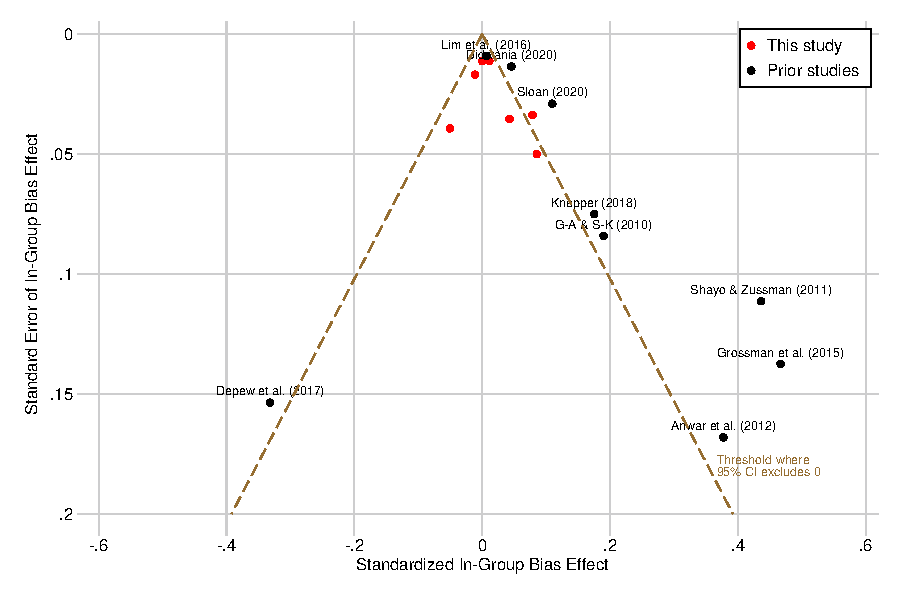
\includegraphics[scale=0.8]{figures/pub_bias.pdf} \\
  \end{center}
   \begin{minipage}{1.0\textwidth}
   \footnotesize \emph{Notes:} This figure shows point estimates of in-group bias from other studies in the relevant literature. From top to bottom, the coefficients of in-group bias (Panel A) correspond to \cite{ShayoZussman2011QJE}, \cite{AnwarBayerHjalmarsson2012TQJoE}, 
    \cite{depew2017judges},
   \cite{knepper2018shadow}, \cite{sloane2019racial}, \cite{Didwania2018CLE}, \cite{lim2016judges}, 
   \cite{gazal2010let}, and the main estimates from the present study respectively. Panel B plots reported bias effects (Y axis) against effect standard errors. All effect sizes are standardized (dividing outcome variables by their standard deviation) to allow comparison across studies.
   % appendix table X describes each study and outcome in more detail
   \par 
   \end{minipage}
\end{figure}

One reason our results stand out from the literature could be publication bias in studies of judicial in-group bias. Figure~\ref{fig:literature} Panel B plots the effect size of each study above against the standard error of the main estimated effect.\footnote{When papers report multiple specifications for the main effect, we used the effect size described most prominently in the text or described by the authors as the ``main specification.'' When papers had multiple outcomes, we used the outcome most similar to the acquittal or conviction rate, as in this study. If these were unavailable, we used the outcome most prominently described in the paper's abstract and introduction.} With the standard error axis reversed, this is the standard ``funnel plot'' used to examine publication bias. In the absence of publication bias or a design-based mechanical correlation (such as adaptive sampling), study estimates should form a cone that is centered around the true estimate \citep{egger1997bias,gerber2001testing,levine2009sample,slavin2009relationship,kuhberger2014publication}.\footnote{A cone shape is expected because studies with larger standard errors should produce a wider range of estimates around the true value.} The set of studies examined here show a highly non-conic and asymmetric shape, where effect magnitude is highly correlated with effect size, such that many of the studies fall just outside the cone boundary defining statistical significance at the 5\% level. While other explanations may be considered, the funnel plot is at least consistent with a substantial degree of publication bias.

Whatever the explanation, our evidence suggests that despite India's deep cleavages and much evidence of discrimination, the state has successfully built a judicial institution where existing disparities are not entrenched by in-group bias among judges. This institutional success should be celebrated, not least because it provides guidance to policymakers in how to allocate resources to address the clear and extant social disparities in Indian society. As a starting point, we have not yet ruled out bias in the broader criminal justice system. %We have focused on a form of bias which has been widely documented in other countries, but it is only one form of potential bias at one stage of the criminal justice pipeline. 
Notwithstanding our results on acquittals, the legal system could still be biased against Muslims and women due to unequal geographic distribution of policing, discrimination in investigations, police/prosecutor decisions to file cases, the severity of charges applied, the severity of penalties imposed, the appeals process, civil litigation, or via other factors. Based on our evidence, these other parts of the justice pipeline might deserve more immediate attention from policymakers than judge acquittal decisions. 

These points also provide some guidance and motivation for social scientists. More research is needed to study the entire justice process in India and other developing countries. That process could start with expansion of the publicly available datasets.

\clearpage


\bibliographystyle{apalike}
\bibliography{elliott,india}

\clearpage

 
\begin{appendices}

\setcounter{figure}{0} 
\renewcommand{\thefigure}{A\arabic{figure}} 
\setcounter{table}{0} \renewcommand{\thetable}{A\arabic{table}} 


\section{Appendix}

\begin{figure}[htp!]
 \centering
 \caption{India eCourts Case Record Sample}
 \includegraphics[width=0.7\textwidth]{figures/ecourts_case_view.png}
 \label{fig:ecourts_case_view}
 \begin{minipage}{1.0\textwidth}
    {\scriptsize \emph{Notes:} The figure displays an anonymized version of a sample court record from \url{https://ecourts.gov.in/} for the District and Sessions Court of Vidisha. The `Petitioner and Advocate' and `Respondent and Advocate' sections contain the litigant names that we use for assigning gender and religion. The `Acts' section contains the data that allows us to discriminate between civil and criminal cases. We use the `Under Section(s)' column to infer the corresponding crime categories.\par}
 \end{minipage}
\end{figure}

\newpage

\begin{figure}[htp!]
 \centering
 \caption{Sample accounting}
 \includegraphics[width=0.7\textwidth]{figures/nomnoml.png}
 \label{fig:nomnoml}
 \begin{minipage}{1.0\textwidth}
    {\scriptsize \emph{Notes:} The figure displays the process through which we arrive at the analysis dataset from the parent dataset of 77 million legal case records. After restricting the sample to criminal cases, matching these criminal cases with our judge dataset, and dropping bail observations, 8.5 million case records remain. For 6 million (6.6 million) records we can then assign the gender (religion) of the judge and defendant using our machine classifier. Further reductions of the sample size, for instance in results Tables \ref{tab:random_female} and \ref{tab:random_muslim}, are due to the inclusion of fixed effects. When during the same court-month/court-year no female \textbf{and} male (or Muslim \textbf{and} non-Muslim) judges were present, observations are dropped.\par}
 \end{minipage}
\end{figure}

\begin{figure}[htp!]
 \centering
 \caption{India eCourts Sample Judge Information inside the Search Engine}
 \includegraphics[width=0.7\textwidth]{figures/ecourts_judge_scraping.png}
 \label{fig:ecourts_judge_scraping}
 \begin{minipage}{1.0\textwidth}
    {\scriptsize \emph{Notes:} Sample view of the eCourts court order search engine. We scraped the judge information implicitly given in the `Court Number' drop-down list of the search mask on -- in this case -- \url{https://services.ecourts.gov.in/ecourtindia_v4_bilingual/cases/s_order.php?state=D&state_cd=1&dist_cd=19} to obtain judge names and tenures.\par}
 \end{minipage}
\end{figure}


\begin{figure}
    \centering
    \caption{Distribution of courts across districts in the analysis sample}
    \includegraphics[width=.7\textwidth]{figures/court_map_rct} 
    \label{fig:court_maps}
     \begin{minipage}{1.0\textwidth}
    {\scriptsize \emph{Notes:} This figure shows the geographical distribution of the trial courts in our sample. Black lines delineate states, and within those the unit of observation for this graphical illustration are districts. Districts marked in white are not included in our analysis.\par}
 \end{minipage}
\end{figure}

\newpage

\begin{table}
  \begin{center}
  \caption{Summary of Name Classifier Training Datasets}
  \label{tab:training}
  {
\def\sym#1{\ifmmode^{#1}\else\(^{#1}\)\fi}
\begin{tabular}{l*{2}{c}}
\hline\hline
\multicolumn{3}{1}{\textit{Panel A: Delhi voter rolls names}}\\
\hline
%&\multicolumn{1}{c}{(1)}&\multicolumn{1}{c}{(2)}\\
Gender&\multicolumn{1}{c}{Instances}&\multicolumn{1}{c}{Percentage}\\
\hline
Female&6,138,337&44.8\% \\
Male&7,556,138&55.2\% \\
\hline
Total&13,694,475&100.0\% \\
\hline
&&\\
\hline\hline
\multicolumn{3}{1}{\textit{Panel B: National Railway exam names}}\\
\hline
%&\multicolumn{1}{c}{(1)}&\multicolumn{1}{c}{(2)}\\
Religion&\multicolumn{1}{c}{Instances}&\multicolumn{1}{c}{Percentage}\\
\hline
Buddhist&1,910&0.1\% \\
Christian&11,194&0.8\% \\
Hindu&1,174,076&84.8\% \\
Muslim&163,861&11.8\% \\
NA&33,882&2.4\% \\
\hline
Total&1,384,923&100.0\% \\
\hline
\end{tabular}
}


  \end{center}
   \begin{minipage}{1.0\textwidth}
    {\scriptsize \emph{Notes:} Panels A \& B of this table show the distribution of identities in the underlying training datasets of the gender and religion LSTM name classification models respectively.\par}
 \end{minipage}
\end{table}

\begin{table}
\begin{center}
  \caption{Outcome variables mapped to dispositions}
  \label{tab:dispositions}
          \resizebox{0.6\linewidth}{!}{
  {
\def\sym#1{\ifmmode^{#1}\else\(^{#1}\)\fi}
\resizebox{\textwidth}{!}{%
\begin{tabular}{@{}lccc@{}}
\hline \hline 
\multicolumn{1}{l}{} & \multicolumn{3}{c}{Mapped Outcome(s)} \\ \cmidrule{2-4}
Disposition Name & Acquitted & Convicted & Decision \\
\hline 
258 crpc [acquitted] & X &  & X \\
%Abated &   & X & X \\
%Absconded &   & X & X \\
%Accepted &   & X & X \\
Acquitted & X &  & X \\
Allowed & X &  & X \\
%Award &   & X & X \\
%Cancelled &   & X & X \\
%Closed &   & X & X \\
Committed &   &  & X \\
%Compounded &   & X & X \\
Compromise &   &  & X \\
%Confession &   & X & X \\
%Converted &   & X & X \\
Convicted &   &  X & X \\
Decided &   &  & X \\
%Died &   & X & X \\
Dismissed &   &  & X \\
%Disposal in lok adalat &   & X & X \\
Disposed &   & & X \\
%Ex-parte &   & X & X \\
%Execution &   & X & X \\
Fine &   &  & X \\
Judgement &   &  & X \\
%Not press &   & X & X \\
Other &   &  & X \\
%Otherwise &   & X & X \\
%P.O. consign &   & X & X \\
%Partly decreed &   & X & X \\
Plead guilty &   & X  & X \\
Prison &   &  X & X \\
%Probation &   & X & X \\
%Quash &   & X & X \\
Referred to lok adalat &   &  & X \\
Reject &   & & X \\
Remanded &   & & X \\
%Settled &   & X & X \\
%Sine die &   & X & X \\
%Stayed &   & X & X \\
Transferred &   &  & X \\
%Untrace &   & X & X \\
Withdrawn &   &  & X \\
 Missing &   &   &   \\ 
\bottomrule
\end{tabular}%
}}}
\end{center}
 \begin{minipage}{1.0\textwidth}
    {\scriptsize \emph{Notes:} This table illustrates the classification of the raw dispositions into our three outcome variables. In the table, no entry corresponds to the default value 0, and X denotes that the corresponding outcome value is set to 1. If a case has a disposition at all, the indicator variable \textit{Decision} equals 1, and 0 otherwise. Conditional on having a disposition, if the disposition is clearly acquitted, the outcome variable \textit{Acquitted} takes the value 1, and 0 otherwise. The outcome variable for \textit{Conviction} has been coded analogously.\par}
 \end{minipage}
\end{table}


\begin{landscape}
\global\pdfpageattr\expandafter{\the\pdfpageattr/Rotate 90}


\begin{table}
      \begin{center}
        \caption{Summary of charges, by gender of defendant}
        \label{tab:summary_gender}
        \resizebox{1\linewidth}{!}{
        {
\def\sym#1{\ifmmode^{#1}\else\(^{#1}\)\fi}
\begin{tabular}{lcccccr}
  \hline\hline
&\multicolumn{1}{c}{(1)}&\multicolumn{1}{c}{(2)}&\multicolumn{1}{c}{(3)}&\multicolumn{1}{c}{(4)}&\multicolumn{1}{c}{(5)}&\multicolumn{1}{r}{(6)}\\
&{Female share}&{Female share/}&{Female}&{Male} &  {Difference} & {Number of cases}\\
&{}&{population share}&{acquittal rate}&{acquittal rate} & {(3) - (4)} & {}\\
\hline
Murder & 0.101 & 0.210 & 0.249 & 0.183 & 0.066 & 1,129,000\\
Sexual assault & 0.085 & 0.177 & 0.275 & 0.235 & 0.040 & 254,928\\
Violent crimes causing hurt & 0.116 & 0.242 & 0.213 & 0.187 & 0.026 & 1,846,000\\
Violent theft/dacoity & 0.079 & 0.165 & 0.170 & 0.148 & 0.022 & 252,046\\
Crimes against women & 0.093 & 0.194 & 0.274 & 0.248 & 0.026 & 725,388\\
Disturbed pub. health/tranquility & 0.063 & 0.131 & 0.096 & 0.075 & 0.021 & 1,852,000\\
Property Crime & 0.106 & 0.221 & 0.184 & 0.158 & 0.026 & 2,558,000\\
Trespass & 0.115 & 0.240 & 0.223 & 0.202 & 0.021 & 339,045\\
Marriage offenses & 0.120 & 0.250 & 0.271 & 0.264 & 0.007 & 326,214\\
Petty theft & 0.103 & 0.215 & 0.180 & 0.149 & 0.031 & 946,890\\
Other crimes & 0.119 & 0.248 & 0.204 & 0.177 & 0.027 & 9,008,000\\
\hline
Total & 0.108 & 0.225 & 0.201 & 0.167 & 0.034 & 17,170,000\\
\hline\hline
\end{tabular}
}
}
    \end{center}
     \begin{minipage}{1.4\textwidth}
    {\scriptsize \emph{Notes:} Column 1 of this table reports the share of female defendants for each crime category. Column 2 reports the ratio of the female share for each crime to the female population share in India. Column 3 reports the acquittal rate for females accused of each crime category. Column 4 reports the analogous acquittal rates for males. Column 5 reports the difference in female and male acquittal rates for each crime category. Column 6 reports the total number of case records in each crime category. The total number of cases in this table is larger than the 6 million cases mentioned in \ref{fig:ecourts_case_view} as we also include cases records in the statistics where only the defendant gender is defined, even if the judge gender is unknown.\par}
 \end{minipage}
\end{table}

\begin{table}
      \begin{center}
        \caption{Summary of charges, by religion of defendant}
        \label{tab:summary_religion}
        \resizebox{1\linewidth}{!}{
        {
\def\sym#1{\ifmmode^{#1}\else\(^{#1}\)\fi}
\begin{tabular}{lcccccr}
  \hline\hline
&\multicolumn{1}{c}{(1)}&\multicolumn{1}{c}{(2)}&\multicolumn{1}{c}{(3)}&\multicolumn{1}{c}{(4)}&\multicolumn{1}{c}{(5)}&\multicolumn{1}{r}{(6)}\\
&{Muslim share}&{Muslim share/}&{Muslim}&{Non-Muslim} &  {Difference} & {Number of cases}\\
&{}&{population share}&{acquittal rate}&{acquittal rate} & {(3) - (4)} & {}\\
\hline
Murder & 0.135 & 0.951 & 0.182 & 0.193 & -0.011 & 1,204,000\\
Sexual assault & 0.163 & 1.148 & 0.241 & 0.238 & 0.003 & 271,622\\
Violent crimes causing hurt & 0.141 & 0.993 & 0.187 & 0.191 & -0.004 & 1,980,000\\
Violent theft/dacoity & 0.194 & 1.366 & 0.140 & 0.152 & -0.012 & 271,901\\
Crimes against women & 0.193 & 1.359 & 0.260 & 0.248 & 0.012 & 771,555\\
Disturbed pub. health/tranquility & 0.164 & 1.155 & 0.078 & 0.075 & 0.003 & 2,002,000\\
Property Crime & 0.165 & 1.162 & 0.161 & 0.161 & 0.000 & 2,711,000\\
Trespass & 0.144 & 1.014 & 0.200 & 0.206 & -0.006 & 362,459\\
Marriage offenses & 0.230 & 1.620 & 0.285 & 0.261 & 0.024 & 344,708\\
Petty theft & 0.180 & 1.268 & 0.153 & 0.153 & 0.000 & 1,003,000\\
Other crimes & 0.136 & 0.958 & 0.195 & 0.178 & 0.017 & 9,556,000\\
\hline
Total & 0.147 & 1.035 & 0.177 & 0.170 & 0.007 & 18,280,000\\
\hline\hline
\end{tabular}
}
}
      \end{center}
        \begin{minipage}{1.4\textwidth}
    {\scriptsize \emph{Notes:} Column 1 of this table reports the share of Muslim defendants for each crime category. Column 2 reports the ratio of the Muslim share for each crime to the Muslim population share in India. Column 3 reports the acquittal rate for Muslims accused of each crime category. Column 4 reports the analogous acquittal rates for non-Muslims. Column 5 reports the difference in Muslim and non-Muslim acquittal rates for each crime category. Column 6 reports the total number of case records in each crime category. The total number of cases in this table is larger than the 6.6 million cases mentioned in \ref{fig:ecourts_case_view} as we also include cases records in the statistics where only the defendant religion is defined, even if the judge religion is unknown.\par}
 \end{minipage}
\end{table}

\end{landscape}
\global\pdfpageattr\expandafter{\the\pdfpageattr/Rotate 0}


% \begin{table}
% \begin{center}
%   \caption{Explanation of coefficients in the primary specification}
%   \label{tab:outcome_coefficient_matrix}
%   \input{tables/outcome_coefficient_matrix.tex}
% \end{center}
%   \begin{minipage}{1\textwidth}
%     {\scriptsize \emph{Notes:} This table explains each coefficient that appears in Equation \ref{eq:random_female}. Specifically, $\beta_{1} + \beta_{2} + \beta_{3} $ represents the effect of random assignment to a male judge for a male defendant on his acquittal likelihood. $\beta_{1}$ represents the effect of random assignment to a male judge for a female defendant on her acquittal likelihood. Similarly, $\beta_{2}$ represents the effect of random assignment to a male judge for a female defendant. If there were own gender bias, we would expect the difference (i.e. $\beta_{3}$) between relative treatment of male judge of male defendants (i.e. $\beta_{2} + \beta_{3}$) and relative treatment of female judge of male defendants (i.e. $\beta_{2}$) to be positive and statistically significant. In this set-up, $\beta_{3}$ represents the magnitude of own-gender bias. The coefficients have analogous meanings in the religion bias analysis specification of Equation \ref{eq:random_muslim}. \par}
%  \end{minipage}
% \end{table}

%% Commented since the RCT sample description says we drop courts with one judge only.
%% \begin{figure}
%%     \centering
%%     \caption{Distribution of court sizes in the analysis samples}
%%     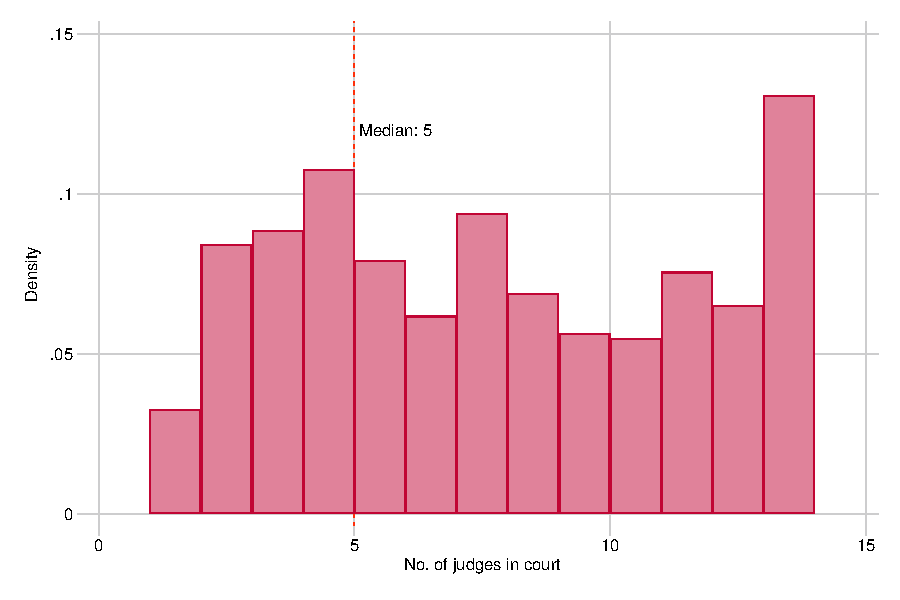
\includegraphics[width=0.9\textwidth]{figures/court_size.png}
%%     \label{fig:court_size}
%%      \begin{minipage}{1.0\textwidth}
%%     {\scriptsize \emph{Notes:} This figure shows the distribution of court sizes in the analysis sample. The smallest courts consist of one judge only, whereas the largest courts comprise up to 14 judges.\par}
%%  \end{minipage}
%% \end{figure}

\begin{landscape}
\global\pdfpageattr\expandafter{\the\pdfpageattr/Rotate 90}

\begin{table}
    \begin{center}
        \caption{Impact of assignment to a male judge on non-conviction}
        \label{tab:app_random_female}
        {
\def\sym#1{\ifmmode^{#1}\else\(^{#1}\)\fi}
\begin{tabular}{l*{6}{c}}
  \hline\hline
\multicolumn{7}{c}{\textit{Outcome variable: Not convicted}}\\
\hline
&\multicolumn{1}{c}{(1)}&\multicolumn{1}{c}{(2)}&\multicolumn{1}{c}{(3)}&\multicolumn{1}{c}{(4)}&\multicolumn{1}{c}{(5)}&\multicolumn{1}{c}{(6)}\\
\hline
Male judge on female defendant \hspace{15mm} & 0.003** & 0.002 & --- & 0.003* & 0.002 & --- \\
& (0.002) & (0.002) &  & (0.002) &(0.002) &  \\
Male judge on male defendant \hspace{15mm} & 0.003** & 0.002 & ---& 0.003* & 0.002 & --- \\
& (0.002) & (0.002) &  & (0.002) & (0.002) &  \\
\textbf{Difference = Own gender bias} \hspace{15mm} & 0.000 & 0.000 & 0.001 & 0.000 & 0.000 & 0.001 \\
& (0.001) & (0.001) & (0.001) & (0.001) & (0.001) & (0.001) \\
\hline
Reference group mean & 0.947 & 0.947 & 0.947 & 0.947 & 0.947 & 0.947 \\
Observations & 5250907 & 5156887 & 5155378 & 5264320 & 5170380 & 5168583 \\
Demographic controls & No & Yes & Yes & No & Yes & Yes \\
Judge fixed effect & No & No & Yes & No & No & Yes \\
Fixed Effect & Court-month & Court-month & Court-month & Court-year & Court-year & Court-year \\
\hline\hline
%\multicolumn{6}{l}{\footnotesize \textit{Standard errors in parentheses}}\\
%\multicolumn{6}{l}{\footnotesize \sym{*} \(p<0.10\), \sym{**} \(p<0.05\), \sym{***} \(p<0.01\)}\\
%\multicolumn{6}{l}{\footnotesize \textit{Reference group: Female judges, female defendants}}\\
%\multicolumn{6}{l}{\footnotesize Specification: \textit{Y_{i,c,t} $=$ \alpha $+$ \beta_{1} \text{judge\_male}_{i,c,t} $+$ \beta_{2} \text{def\_male}_{i,c,t}  $+$  \beta_{3} \text{judge\_male}_{i,c,t}\sym{*}\text{def\_male}_{i,c,t} $+$ \phi_{c,t} $+$ \delta \chi_{i,c,t} $+$ \epsilon}}\\
\end{tabular}
}
 

    \end{center}
    \begin{minipage}{1.6\textwidth}
        \footnotesize 
        \emph{Notes:} Standard errors in parentheses. \sym{*} \(p<0.10\), \sym{**} \(p<0.05\), \sym{***} \(p<0.01\).  \par 
        Reference group: Female judges, female defendants.  \par
        Charge section fixed effects have been used across all columns reported. \par
        Specification: $Y_{i,s,c,t} = \beta_{1} \text{judgeMale}_{i,s,c,t} + \beta_{2} \text{defMale}_{i,s,c,t} + \beta_{3} \text{judgeMale}_{i,s,c,t} * \text{defMale}_{i,s,c,t} + \phi_{c,t} + \zeta_{s} + \delta \chi_{i,s,c,t} + \epsilon_{i,s,c,t}$ \par
   \end{minipage}
\end{table}


\begin{table}
  \begin{center}
     \caption{Impact of assignment to a male judge on acquittal rates, dropping ambiguous outcomes}
      \label{tab:amb_random_female}
     {
\def\sym#1{\ifmmode^{#1}\else\(^{#1}\)\fi}
\begin{tabular}{l*{6}{c}}
  \hline\hline
\multicolumn{7}{c}{\textit{Outcome variable: Acquittal rate}}\\
\hline
&\multicolumn{1}{c}{(1)}&\multicolumn{1}{c}{(2)}&\multicolumn{1}{c}{(3)}&\multicolumn{1}{c}{(4)}&\multicolumn{1}{c}{(5)}&\multicolumn{1}{c}{(6)}\\
\hline
Male judge on female defendant \hspace{15mm} & -0.003 & -0.008 & --- & -0.005 & -0.009* & --- \\
& (0.005) & (0.005) &  & (0.004) &(0.005) &  \\
Male judge on male defendant \hspace{15mm} & 0.000 & -0.005 & ---& -0.001 & -0.006 & --- \\
& (0.004) & (0.005) &  & (0.004) & (0.004) &  \\
\textbf{Difference = Own gender bias} \hspace{15mm} & 0.002 & 0.003 & 0.004 & 0.003 & 0.003 & 0.004 \\
& (0.003) & (0.003) & (0.003) & (0.003) & (0.003) & (0.003) \\
\hline
Reference group mean & 0.663 & 0.664 & 0.664 & 0.666 & 0.666 & 0.666 \\
Observations & 1182938 & 1162073 & 1159551 & 1203939 & 1183155 & 1180587 \\
Demographic controls & No & Yes & Yes & No & Yes & Yes \\
Judge fixed effect & No & No & Yes & No & No & Yes \\
Fixed Effect & Court-month & Court-month & Court-month & Court-year & Court-year & Court-year \\
\hline\hline
%\multicolumn{6}{l}{\footnotesize \textit{Standard errors in parentheses}}\\
%\multicolumn{6}{l}{\footnotesize \sym{*} \(p<0.10\), \sym{**} \(p<0.05\), \sym{***} \(p<0.01\)}\\
%\multicolumn{6}{l}{\footnotesize \textit{Reference group: Female judges, female defendants}}\\
%\multicolumn{6}{l}{\footnotesize Specification: \textit{Y_{i,c,t} $=$ \alpha $+$ \beta_{1} \text{judge\_male}_{i,c,t} $+$ \beta_{2} \text{def\_male}_{i,c,t}  $+$  \beta_{3} \text{judge\_male}_{i,c,t}\sym{*}\text{def\_male}_{i,c,t} $+$ \phi_{c,t} $+$ \delta \chi_{i,c,t} $+$ \epsilon}}\\
\end{tabular}
}
 

    \end{center}
    \begin{minipage}{1.6\textwidth}
        \footnotesize 
        \emph{Notes:} Standard errors in parentheses. \sym{*} \(p<0.10\), \sym{**} \(p<0.05\), \sym{***} \(p<0.01\).  \par 
        Reference group: Female judges, female defendants.  \par
        Charge section fixed effects have been used across all columns reported. \par
        Specification: $Y_{i,s,c,t} = \beta_{1} \text{judgeMale}_{i,s,c,t} + \beta_{2} \text{defMale}_{i,s,c,t} + \beta_{3} \text{judgeMale}_{i,s,c,t} * \text{defMale}_{i,s,c,t} + \phi_{c,t} + \zeta_{s} + \delta \chi_{i,s,c,t} + \epsilon_{i,s,c,t}$ \par
   \end{minipage}
\end{table}

\begin{table}
  \begin{center}
     \caption{Impact of assignment to a male judge on whether the disposition is ambiguous}
      \label{tab:robust_amb_female}
     {
\def\sym#1{\ifmmode^{#1}\else\(^{#1}\)\fi}
\begin{tabular}{l*{6}{c}}
  \hline\hline
\multicolumn{7}{c}{\textit{Outcome variable: Ambiguous outcome}}\\
\hline
&\multicolumn{1}{c}{(1)}&\multicolumn{1}{c}{(2)}&\multicolumn{1}{c}{(3)}&\multicolumn{1}{c}{(4)}&\multicolumn{1}{c}{(5)}&\multicolumn{1}{c}{(6)}\\
\hline
Male judge on female defendant \hspace{15mm} & 0.011*** & 0.008** & --- & 0.010*** & 0.007** & --- \\
& (0.003) & (0.004) &  & (0.003) &(0.004) &  \\
Male judge on male defendant \hspace{15mm} & 0.011*** & 0.008** & ---& 0.010*** & 0.007** & --- \\
& (0.003) & (0.003) &  & (0.003) & (0.003) &  \\
\textbf{Difference = Own gender bias} \hspace{15mm} & 0.000 & 0.000 & 0.002 & 0.000 & 0.000 & 0.003 \\
& (0.002) & (0.002) & (0.002) & (0.002) & (0.002) & (0.002) \\
\hline
Reference group mean & 0.737 & 0.736 & 0.736 & 0.737 & 0.735 & 0.735 \\
Observations & 5250907 & 5156887 & 5155378 & 5264320 & 5170380 & 5168583 \\
Demographic controls & No & Yes & Yes & No & Yes & Yes \\
Judge fixed effect & No & No & Yes & No & No & Yes \\
Fixed Effect & Court-month & Court-month & Court-month & Court-year & Court-year & Court-year \\
\hline\hline
%\multicolumn{6}{l}{\footnotesize \textit{Standard errors in parentheses}}\\
%\multicolumn{6}{l}{\footnotesize \sym{*} \(p<0.10\), \sym{**} \(p<0.05\), \sym{***} \(p<0.01\)}\\
%\multicolumn{6}{l}{\footnotesize \textit{Reference group: Female judges, female defendants}}\\
%\multicolumn{6}{l}{\footnotesize Specification: \textit{Y_{i,c,t} $=$ \alpha $+$ \beta_{1} \text{judge\_male}_{i,c,t} $+$ \beta_{2} \text{def\_male}_{i,c,t}  $+$  \beta_{3} \text{judge\_male}_{i,c,t}\sym{*}\text{def\_male}_{i,c,t} $+$ \phi_{c,t} $+$ \delta \chi_{i,c,t} $+$ \epsilon}}\\
\end{tabular}
}
 

    \end{center}
    \begin{minipage}{1.6\textwidth}
        \footnotesize 
        \emph{Notes:} Standard errors in parentheses. \sym{*} \(p<0.10\), \sym{**} \(p<0.05\), \sym{***} \(p<0.01\).  \par 
        Reference group: Female judges, female defendants.  \par
        Charge section fixed effects have been used across all columns reported. \par
        Specification: $Y_{i,s,c,t} = \beta_{1} \text{judgeMale}_{i,s,c,t} + \beta_{2} \text{defMale}_{i,s,c,t} + \beta_{3} \text{judgeMale}_{i,s,c,t} * \text{defMale}_{i,s,c,t} + \phi_{c,t} + \zeta_{s} + \delta \chi_{i,s,c,t} + \epsilon_{i,s,c,t}$ \par
   \end{minipage}
\end{table}

\begin{table}
  \begin{center}
     \caption{Impact of assignment to a non-Muslim judge on non-conviction}
      \label{tab:app_random_muslim}
     {
\def\sym#1{\ifmmode^{#1}\else\(^{#1}\)\fi}
\begin{tabular}{l*{6}{c}}
  \hline\hline
\multicolumn{7}{c}{\textit{Outcome variable: Not convicted}}\\
\hline
&\multicolumn{1}{c}{(1)}&\multicolumn{1}{c}{(2)}&\multicolumn{1}{c}{(3)}&\multicolumn{1}{c}{(4)}&\multicolumn{1}{c}{(5)}&\multicolumn{1}{c}{(6)}\\
\hline
Non-Muslim judge on Muslim defendant \hspace{15mm}& 0.002 & -0.003 & --- & 0.001 & -0.004 & --- \\
& (0.003) & (0.003) &  & (0.003) &(0.003) &  \\
Non-Muslim judge on non-Muslim defendant \hspace{15mm}& 0.005 & 0.001 & ---& 0.005 & 0.001 & --- \\
& (0.003) & (0.003) &  & (0.004) & (0.003) &  \\
\textbf{Difference = Own religion bias} & 0.003* & 0.004** & 0.003* & 0.004* & 0.005** & 0.003** \\
& (0.002) & (0.002) & (0.002) & (0.002) & (0.003) & (0.002) \\
\hline
Reference group mean & 0.936 & 0.937 & 0.937 & 0.937 & 0.938 & 0.938 \\
Observations & 5684426 & 5241649 & 5240140 & 5697480 & 5255137 & 5253328 \\
Demographic controls & No & Yes & Yes & No & Yes & Yes \\
Judge fixed effect & No & No & Yes & No & No & Yes \\
Fixed Effect & Court-month & Court-month & Court-month & Court-year & Court-year & Court-year \\
\hline\hline
\end{tabular}
}
 

    \end{center}
    \begin{minipage}{1.6\textwidth}
        \footnotesize 
        \emph{Notes:} Standard errors in parentheses. \sym{*} \(p<0.10\), \sym{**} \(p<0.05\), \sym{***} \(p<0.01\).  \par 
        Reference group: Muslim judges, Muslim defendants.  \par
        Charge section fixed effects have been used across all columns reported. \par
        Specification: $Y_{i,s,c,t} = \beta_{1} \text{judgeNonMuslim}_{i,s,c,t} + \beta_{2} \text{defNonMuslim}_{i,s,c,t} + \beta_{3} \text{judgeNonMuslim}_{i,s,c,t} * \text{defNonMuslim}_{i,s,c,t} + \phi_{c,t} + \zeta_{s} + \delta \chi_{i,s,c,t} + \epsilon_{i,s,c,t}$  \par
   \end{minipage}
\end{table}


\begin{table}
  \begin{center}
     \caption{Impact of assignment to a non-Muslim judge on acquittal rates,  dropping ambiguous outcomes}
      \label{tab:amb_random_muslim}
     {
\def\sym#1{\ifmmode^{#1}\else\(^{#1}\)\fi}
\begin{tabular}{l*{6}{c}}
  \hline\hline
\multicolumn{7}{c}{\textit{Outcome variable: Acquittal rate}}\\
\hline
&\multicolumn{1}{c}{(1)}&\multicolumn{1}{c}{(2)}&\multicolumn{1}{c}{(3)}&\multicolumn{1}{c}{(4)}&\multicolumn{1}{c}{(5)}&\multicolumn{1}{c}{(6)}\\
\hline
Non-Muslim judge on Muslim defendant \hspace{15mm}& 0.010 & 0.000 & --- & 0.007 & -0.006 & --- \\
& (0.006) & (0.008) &  & (0.006) &(0.007) &  \\
Non-Muslim judge on non-Muslim defendant \hspace{15mm}& 0.010* & 0.002 & ---& 0.009 & -0.002 & --- \\
& (0.006) & (0.007) &  & (0.006) & (0.007) &  \\
\textbf{Difference = Own religion bias} & 0.000 & 0.002 & -0.002 & 0.002 & 0.004 & 0.000 \\
& (0.005) & (0.005) & (0.004) & (0.005) & (0.005) & (0.004) \\
\hline
Reference group mean & 0.676 & 0.682 & 0.682 & 0.677 & 0.683 & 0.683 \\
Observations & 1285585 & 1187003 & 1184449 & 1306413 & 1208242 & 1205650 \\
Demographic controls & No & Yes & Yes & No & Yes & Yes \\
Judge fixed effect & No & No & Yes & No & No & Yes \\
Fixed Effect & Court-month & Court-month & Court-month & Court-year & Court-year & Court-year \\
\hline\hline
\end{tabular}
}
 

    \end{center}
    \begin{minipage}{1.6\textwidth}
        \footnotesize 
        \emph{Notes:} Standard errors in parentheses. \sym{*} \(p<0.10\), \sym{**} \(p<0.05\), \sym{***} \(p<0.01\).  \par 
        Reference group: Muslim judges, Muslim defendants.  \par
        Charge section fixed effects have been used across all columns reported. \par
        Specification: $Y_{i,s,c,t} = \beta_{1} \text{judgeNonMuslim}_{i,s,c,t} + \beta_{2} \text{defNonMuslim}_{i,s,c,t} + \beta_{3} \text{judgeNonMuslim}_{i,s,c,t} * \text{defNonMuslim}_{i,s,c,t} + \phi_{c,t} + \zeta_{s} + \delta \chi_{i,s,c,t} + \epsilon_{i,s,c,t}$  \par
   \end{minipage}
\end{table}

\begin{table}
  \begin{center}
     \caption{Impact of assignment to a non-Muslim judge on whether the disposition is ambiguous}
      \label{tab:robust_amb_Muslim}
     {
\def\sym#1{\ifmmode^{#1}\else\(^{#1}\)\fi}
\begin{tabular}{l*{6}{c}}
  \hline\hline
\multicolumn{7}{c}{\textit{Outcome variable: Ambiguous outcome}}\\
\hline
&\multicolumn{1}{c}{(1)}&\multicolumn{1}{c}{(2)}&\multicolumn{1}{c}{(3)}&\multicolumn{1}{c}{(4)}&\multicolumn{1}{c}{(5)}&\multicolumn{1}{c}{(6)}\\
\hline
Non-Muslim judge on Muslim defendant \hspace{15mm}& -0.006 & -0.013 & --- & -0.006 & -0.013 & --- \\
& (0.005) & (0.006) &  & (0.005) &(0.006) &  \\
Non-Muslim judge on non-Muslim defendant \hspace{15mm}& -0.002 & -0.008 & ---& -0.002 & -0.008 & --- \\
& (0.005) & (0.006) &  & (0.005) & (0.006) &  \\
\textbf{Difference = Own religion bias} & 0.004 & 0.005 & 0.001 & 0.005 & 0.005 & 0.001 \\
& (0.004) & (0.004) & (0.003) & (0.004) & (0.004) & (0.003) \\
\hline
Reference group mean & 0.735 & 0.732 & 0.732 & 0.734 & 0.732 & 0.732 \\
Observations & 5684426 & 5241649 & 5240140 & 5697480 & 5255137 & 5253328 \\
Demographic controls & No & Yes & Yes & No & Yes & Yes \\
Judge fixed effect & No & No & Yes & No & No & Yes \\
Fixed Effect & Court-month & Court-month & Court-month & Court-year & Court-year & Court-year \\
\hline\hline
\end{tabular}
}
 

    \end{center}
    \begin{minipage}{1.6\textwidth}
        \footnotesize 
        \emph{Notes:} Standard errors in parentheses. \sym{*} \(p<0.10\), \sym{**} \(p<0.05\), \sym{***} \(p<0.01\).  \par 
        Reference group: Muslim judges, Muslim defendants.  \par
        Charge section fixed effects have been used across all columns reported. \par
        Specification: $Y_{i,s,c,t} = \beta_{1} \text{judgeNonMuslim}_{i,s,c,t} + \beta_{2} \text{defNonMuslim}_{i,s,c,t} + \beta_{3} \text{judgeNonMuslim}_{i,s,c,t} * \text{defNonMuslim}_{i,s,c,t} + \phi_{c,t} + \zeta_{s} + \delta \chi_{i,s,c,t} + \epsilon_{i,s,c,t}$  \par
   \end{minipage}
\end{table}

\begin{table}[ht!]
      \begin{center}
        \caption{Impact of assignment to a male judge when the offence was a crime against women}
        \label{tab:crime_women}
        {
\def\sym#1{\ifmmode^{#1}\else\(^{#1}\)\fi}
\begin{tabular}{l*{6}{c}}
  \hline\hline
\multicolumn{7}{c}{\textit{Outcome variable: Acquittal rate}}\\
\hline
&\multicolumn{1}{c}{(1)}&\multicolumn{1}{c}{(2)}&\multicolumn{1}{c}{(3)}&\multicolumn{1}{c}{(4)}&\multicolumn{1}{c}{(5)}&\multicolumn{1}{c}{(6)}\\
\hline
Male judge on female defendant \hspace{15mm} & -0.027*** & -0.018* & --- & -0.029*** & -0.020** & --- \\
& (0.009) & (0.010) &  & (0.008) &(0.009) &  \\
Male judge on male defendant \hspace{15mm} & -0.028*** & -0.021*** & ---& -0.025*** & -0.018*** & --- \\
& (0.005) & (0.007) &  & (0.005) & (0.007) &  \\
\textbf{Difference = Own gender bias} \hspace{15mm} & -0.001 & -0.003 & -0.004 & 0.004 & 0.002 & 0.003 \\
& (0.008) & (0.008) & (0.008) & (0.007) & (0.007) & (0.007) \\
\hline
Reference group mean & 0.27 & 0.27 & 0.27 & 0.276 & 0.276 & 0.277 \\
Observations & 261459 & 258216 & 255314 & 280236 & 276998 & 273964 \\
Demographic controls & No & Yes & Yes & No & Yes & Yes \\
Judge fixed effect & No & No & Yes & No & No & Yes \\
Fixed Effect & Court-month & Court-month & Court-month & Court-year & Court-year & Court-year \\
\hline\hline
%\multicolumn{6}{l}{\footnotesize \textit{Standard errors in parentheses}}\\
%\multicolumn{6}{l}{\footnotesize \sym{*} \(p<0.10\), \sym{**} \(p<0.05\), \sym{***} \(p<0.01\)}\\
%\multicolumn{6}{l}{\footnotesize \textit{Reference group: Female judges, female defendants}}\\
%\multicolumn{6}{l}{\footnotesize Specification: \textit{Y_{i,c,t} $=$ \alpha $+$ \beta_{1} \text{judge\_male}_{i,c,t} $+$ \beta_{2} \text{def\_male}_{i,c,t}  $+$  \beta_{3} \text{judge\_male}_{i,c,t}\sym{*}\text{def\_male}_{i,c,t} $+$ \phi_{c,t} $+$ \delta \chi_{i,c,t} $+$ \epsilon}}\\
\end{tabular}
}
 

      \end{center}
    \begin{minipage}{1.6\textwidth}
        \footnotesize 
        \emph{Notes:} Standard errors in parentheses. \sym{*} \(p<0.10\), \sym{**} \(p<0.05\), \sym{***} \(p<0.01\).  \par 
        Reference group: Female judges, female defendants.  \par
        Charge section fixed effects have been used across all columns reported. \par
        Specification: $Y_{i,s,c,t} = \beta_{1} \text{judgeMale}_{i,s,c,t} + \beta_{2} \text{defMale}_{i,s,c,t} + \beta_{3} \text{judgeMale}_{i,s,c,t} * \text{defMale}_{i,s,c,t} + \phi_{c,t} + \zeta_{s} + \delta \chi_{i,s,c,t} + \epsilon_{i,s,c,t}$ \par
   \end{minipage}
\end{table}
% \sym{*} \(p<0.10\), \sym{**} \(p<0.05\), \sym{***} \(p<0.01\)

\end{landscape}
\global\pdfpageattr\expandafter{\the\pdfpageattr/Rotate 0}

%% \begin{figure}
%%       \centering
%%       \caption{Heterogeneity analysis of in-group bias, by crime category}
%%       \label{fig:crime_type}
%%             \begin{tabular}{@{}ll@{}}
%%         \includegraphics[width=.5\textwidth]{figures/gender_crime_coef.png} &
%%         \includegraphics[width=.5\textwidth]{figures/religion_crime_coef.png} \\
%%       \end{tabular}
%%       
%%   \begin{minipage}{1.0\textwidth}
%%     {\scriptsize \emph{Notes:} Each coefficient is drawn from the following regression specification for subsamples of specific crime categories:  $Y_{i,s,c,t} = \beta_{1} \text{judge[Male/NonMuslim]}_{i,s,c,t} + \beta_{2} \text{def[Male/NonMuslim]}_{i,s,c,t} + \beta_{3} \text{judge[Male/NonMuslim]}_{i,s,c,t} * \text{def[Male/NonMuslim]}_{i,s,c,t} + \phi_{c,t} + \zeta_{s} + \delta \chi_{i,s,c,t} + \epsilon_{i,s,c,t}$
%%     Court-month, charge section and judge fixed effects are applied throughout. The coefficients represented in the figure correspond to $\beta_{3}$ in the specification. $\beta_{3}$ represents in-group gender bias in Panel A and in-group religious bias in Panel B, for each subsample.\par}
%%    \end{minipage}
%%   \end{figure}
  

\end{appendices}
\end{document}
